\documentclass{kththesis}

\usepackage{minted}

\usepackage{syntax}
\usepackage{tabu}
\usepackage{amsmath}
\usepackage{semantic}
\usepackage{graphicx}
\usepackage{parskip}
\usepackage{afterpage}

\usepackage{algpseudocode}

\usepackage{csquotes} % Recommended by biblatex
\usepackage[doi=false,url=false]{biblatex}
\addbibresource{references.bib} % The file containing our references, in BibTeX format

\usepackage{hyperref}

\newmintinline[syncon]{syncon}{}
\setminted{
frame=single
}

\title{Building Programming Languages, Construction by Construction}
\alttitle{Att bygga programmeringsspråk, konstruktion för konstruktion}
\author{Viktor Palmkvist}
\email{vipa@kth.se}
\supervisor{David Broman}
\examiner{Mads Dam}
\programme{Master in Computer Science}
\school{School of Computer Science and Communication}
\date{\today}


\raggedright
% \setlength{\parindent}{1.5em}

\hyphenation{conclusion}

\newcommand{\ssynt}[1]{\ensuremath{\mathit{#1}}}
\newenvironment{sgrammar}{\begin{grammar}\renewcommand{\grammarlabel}[2]{\ssynt{##1} \hfill##2}}{\end{grammar}}

\begin{document}

% Frontmatter includes the titlepage, abstracts and table-of-contents
\frontmatter

\titlepage

\begin{abstract}
The task of implementing a programming language is a task that entails a great deal of work. Yet much of this work is similar for different programming languages: most languages require, e.g., parsing, name resolution, type-checking and optimization. When implementing domain-specific languages (DSLs) the re-implementation of these largely similar tasks seems especially redundant.

A number of approaches exist to alleviate this issue, including embedded DSLs, macro-rewriting systems, and more general systems intended for language implementation. However, these tend to have at least one of the following limitations:

\begin{itemize}
  \item They present a leaky abstraction, e.g., error messages do not refer to the DSL but rather some other programming language, namely the one used to implement the DSL.
  \item They limit the flexibility of the DSL, either to the constructs present in another language, or merely to the syntax of some other language.
  \item They see an entire language as the unit of composition. Complete languages are extended with other complete language extensions.
\end{itemize}

Instead, this thesis introduces the concept of a syntax construction, which represents a smaller unit of composition. A syntax construction defines a single language feature, e.g., an if-statement, an anonymous function, or addition. Each syntax construction specifies its own syntax, binding semantics, and runtime semantics, independent of the rest of the language. The runtime semantics are defined using a translation into another target language, similarly to macros. These translations can then be checked to ensure that they preserve binding semantics and introduce no binding errors. This checking ensures that binding errors can be presented in terms of code the programmer wrote, rather than generated code in some underlying language.

\enlargethispage{\baselineskip}

During evaluation several limitations are encountered. Removing or minimizing these limitations appears possible, but is left for future work.
\end{abstract}

\begin{otherlanguage}{swedish}
\begin{abstract}
Denna avhandling introducerar syntax-konstruktioner, en metod för att konstruera programmeringsspråk som en samling mindre konstruktioner. Detta gör det möjligt att återanvända enstaka konstruktioner från redan implementerade språk. Syntax-konstruktioner liknar macron, men med större syntaktisk flexibilitet och ett sätt att specificera hur de interagerar med namnbindning. Det sistnämnda möjliggör analys av namnbindningar utan att expandera macron och ett sätt att kontrollera att en given macro aldrig introducerar namnbindningsfel. Detta medför att när felmeddelanden behöver presenteras så kan de referera till kod som en användare faktiskt skrivit, istället för kod som genererats vid expandering.

Syntax-konstruktioner låter en användare skapa syntaktisk ambiguitet i sitt programmeringsspråk och försöker få en bra användarupplevelse med hjälp av informativa felmeddelanden. De verktyp som tillhandahålls för att kontrollera detta visar sig dock vara otillräckliga, vilket medför att syntax-konstruktioner i sig själva inte är en tillräcklig lösning för den tilltänkta användarupplevelsen vid programspråkskonstruktion, utan enbart ett steg på vägen.
\end{abstract}
\end{otherlanguage}


\tableofcontents


% Mainmatter is where the actual contents of the thesis goes
\mainmatter

\chapter{Introduction} \label{sec:introduction}

A domain-specific programming language (DSL) is a programming language created to solve problems in some particular domain. There are numerous methods for creating such languages. A few examples include:

\begin{description}
  \item[Embedded DSLs.] An embedded DSL is a language designed as a library in a host programming language. They use the already existing capabilities of the host language, e.g., name binding, type systems, and other libraries. Some examples include Paradise \cite{Augustsson2008Paradise:-A-Two}, RSpec\footnote{http://rspec.info/}, and Rake\footnote{https://ruby.github.io/rake/}.

  However, embedding a DSL limits it to the capabilities of the host language. Additionally, any type errors produced on incorrect usage may refer to concepts in the host language, rather than the DSL.

  \item[External DSLs.] On the other hand, an external DSL is implemented from the ground up. It is not part of a host language. Examples include CSS, SQL, and DOT\footnote{http://graphviz.org/}.

  While these DSLs are not limited by some host language, they also have no host language to take advantage of. Any capabilities that might have been provided by a host language must instead be re-implemented.

  \item[Macros.] Macros, commonly featured in Lisp dialects, are syntax transformations that run at compile-time. From a practical stand point they allow a programmer to extend a language with new constructs that appear as though they are built in to the language, but are in fact implemented by some translation to the underlying language. They can be used to implement an embedded DSL.

  This gives greater freedom than most other forms of embedded DSLs, but error messages are still likely to refer to the host language, and the syntax is still constrained to that of the host language; a Lisp macro still looks like Lisp.

  \item[Language-definition languages.] This category is somewhat looser defined than the others, but refers to systems whose (primary or secondary) purpose is the construction of programming languages. Some examples include SoundX \cite{Lorenzen2016Sound-type-depe}, Silver \cite{Van-Wyk2010Silver:-An-exte}, and Racket \cite{Tobin-Hochstadt:2011:LL:1993498.1993514}.

  The trade-offs vary by system, but they all tend to consider a language as the base building block when we want to reuse or extend a language: extend a full language with a full language extension.
\end{description}

% discuss embedded DSL, external DSL, costs, weaknesses, probably reusability (?)
% probably start from general-purpose vs domain-specific

This thesis falls under the language-definition language category, but takes a different approach. We introduce \emph{syntax constructions}, which center around singular language constructs. A syntax construction could for example implement an if-statement, an anonymous function, or a pattern used in pattern matching. Each syntax construction describes its own syntax, its binding semantics, and its runtime semantics, independent of other parts of the language. The runtime semantics are specified in terms of a translation to another programming language, and this translation is checked to ensure that it always preserves the binding semantics.

An alternative angle is to consider syntax constructions as macros with some extra features: greater syntactical flexibility and the ability to reason about name bindings without macro expansion. This means that binding errors do \emph{not} refer to the host language.

The self-contained nature of a syntax construction enables creating new programming languages by cherry-picking individual features from previous languages, i.e., it enables reuse of a single language feature as opposed to an entire language. The unit of composition is a feature, not a language.

The remainder of this introduction will provide additional context and motivation for the thesis and the associated approach (Sections \ref{sec:compiler-design} through \ref{sec:desired-ambiguity}), a more precise problem statement (Section~\ref{sec:research-question}), and a list of contributions (Section~\ref{sec:contributions}).

\section{Programming Language Implementation} \label{sec:compiler-design}

The implementation of a programming language---be it an interpreter or a compiler---tends to be divided into phases, each dealing with their own aspect of the language. For example, a parser details the syntax of the language, while name resolution handles names, scoping, and namespaces. A type checker details part of the semantics, what language constructs can be combined, then code generation or a simple interpreter codify the runtime semantics of the individual constructs. This means that the implementation of any single language construct is spread throughout the language implementation, necessitating it be considered as a whole. Adding a new construction requires changes in many places.

This also means that reuse of a language implementation is difficult; each phase makes assumptions on what has been done before it and what will be done later. Trying to use or replace a single phase gives little flexibility to make something different than what is already there.

Attempting to use a single language construct from a language is likewise difficult. The various aspects of its definition are spread throughout the different phases, quite possibly intertwined with code handling other constructs that happen to be similar in that particular language.

Despite this, there are some quite successful cases of language implementation reuse:

\begin{description}
  \item[JVM.] A large number of programming languages exists that can compile to Java bytecode, enabling them to reuse the implementation originally intended for Java. Examples include Scala, Clojure, and Kotlin. Other languages have the JVM as an additional backend, for example Ruby (JRuby) and Python (Jython). % TODO: refs
  \item[JavaScript.] Many languages can compile to JavaScript, thus reusing the entire language while adding something new on top. Examples include TypeScript (essentially JavaScript with static types), CoffeeScript (alternative syntax for JavaScript), and Elm (statically typed language with JavaScript as a compile target).
  \item[OCaml.] ReasonML replaces the parser and surrounding tooling of OCaml, providing a different syntax to what is otherwise the same language.
  \item[LLVM.] The LLVM project (previously an acronym for ''low level virtual machine,'' now a name all by itself) defines an intermediate representation that can be used both as a target for a language and as a source for translation into machine code. This allows changing either frontend or backend while reusing the other, as well as a large number of optimizations defined on the intermediate representation. Languages using LLVM either by default or as part of an alternative backend include C, C++, Rust, and Haskell. Examples of instruction sets to which LLVM intermediate representation can be translated include x86, x86-64, ARM, and PowerPC.

  \item[.NET Framework.] The .NET framework provides a common framework for interoperability between multiple programming languages. This is done by offering a single intermediate language called Common Intermediate Language (more commonly CIL), similar to Java bytecode.
\end{description}

Somewhat simplified, the key common characteristic of these examples is that the reused part tends to be from somewhere in the middle until the end of the original implementation; the replaced part has the first few phases, then all remaining phases are from the original implementation. No one only replaces a few phases in the middle.

While this does allow reuse of large chunks of an implementation, much still has to be reimplemented. The different implementations of the first phases generally do much of the same work, all of them parse their language, then do name resolution, then maybe some type checking, and so on. Many details will differ, but the basic kind of work tends to stay the same.

We would ideally like to have more flexible forms of reuse, enabling reuse of singular language features, and not requiring reimplementation of name resolution and many other common tasks beyond specifying the particular details of the current language.

\section{Macros} \label{sec:introduction-macros}

From a practical viewpoint, a macro is essentially syntax that appears as though it were built in to the programming language, but is in fact defined by a user through a translation to some other syntax. The following example is in Racket~\cite{Flatt2010Reference:-Rack}, a Lisp dialect:

% TODO: check that the example code is actually correct and runnable
\begin{minted}{racket}
; define-syntax-rule introduces a new macro,
; in this case with the name 'and'.
; This is a shortcutting 'and', i.e., 'b' will
; only be evaluated if 'a' is true
(define-syntax-rule (and a b)
  (if a b #f))

; Assuming the existence of a function trace
; that prints its argument and then returns
; it, we can demonstrate 'and' like so:
(and (trace #t) (trace #f))
; => #f
; This prints #t, but not #f, i.e., (trace #f)
; was not evaluated
\end{minted}

This would not be possible to implement as a function in Racket since functions require their arguments to be fully evaluated before they are called, i.e., the second argument would be evaluated before \mintinline{racket}{and}, regardless of the value of the first argument.

This particular example shows a simple example where the arguments of the macro are simply inserted into a form of template, but macros in general can be far more complex and powerful. Macros can utilize recursion as well as the full power of Lisp, i.e., a macro in general is a function from syntax to syntax that runs at compile-time.

The expressive power provided here is great; any arbitrary computation can be done at compile time. Examples include type checking (typed racket \cite{Tobin-Hochstadt:2011:LL:1993498.1993514}), destructuring and pattern matching (Clojure, standard library\footnote{https://github.com/clojure/clojure/blob/master/src/clj/clojure/core.clj} and external library\footnote{https://github.com/clojure/core.match} respectively), and coroutines (Clojure\footnote{https://github.com/clojure/core.async}). Racket (which was used in the example above) takes this one step further and describes itself as an ''ecosystem for developing and deploying new languages'', all of which is powered by its macro system.

There are some drawbacks, however, and we will spend the next few sections examining some of them.

\subsection{Problems of Abstraction} \label{sec:problem-abstraction}

The abstractions provided by macros can easily become leaky abstractions without special care. By leaky abstraction we mean an abstraction that might in some case expose its implementation to a user, or one that cannot be reasoned about correctly without knowing its implementation.

\subsubsection{Name Capture}

A naive macro expander using textual replacement can introduce accidental name capture. For example, given the following macro (using Racket syntax) intended to calculate $a + a + b$:

\begin{minted}{racket}
(define-syntax-rule (double-add a b)
; let introduces a new binding, in this case
; 'x' is bound to the value of evaluating 'a'
  (let ([x a])
    (+ x x b)))
\end{minted}

The extra \mintinline{racket}{let}-binding is there to ensure we only compute \mintinline{racket}{a} once. Macros are expanded at compile-time and receives its arguments as expressions, i.e., they are not values, but rather computations that produce values. The more obvious implementation, \mintinline{racket}{(+ a a b)}, would
compute \mintinline{racket}{a} twice.

The following expression will exhibit accidental name capture when macro expansion uses pure textual replacement:

\begin{minted}{racket}
(let ([x 2])
  (double-add 1 x))
; expands to:
(let ([x 2])
  (let ([x 1])
    (+ x x x)))
; which evaluates to
(+ 1 1 1) = 3
; while our intended semantics would evaluate to:
(+ 1 1 2) = 4
\end{minted}

Notable here is that the above would not produce an error of any kind, the result would simply be silently wrong.

It is worth noting here that Racket solves this problem, as do most other macro systems, through rewriting or more complicated forms of name resolution (e.g., \cite{FLATT2012Macros-that-Wor,Flatt2016Binding-As-Sets}). A notable exception is the C preprocessor that makes no such attempt.

\subsubsection{Errors after Expansion}

In some cases, the fully expanded code is incorrect, either because the macro was poorly implemented, or because it was used improperly. For example:

\begin{minted}{racket}
(define-syntax-rule (new-let x e body)
  (let ([x e])
    body))

(new-let 2 x
  (+ 1 x))
\end{minted}

Here we define a new binding construction, but misuse it; the identifier and the value are switched. The macro expansion will succeed and produce the code below, but at that point an error message will be produced about improper use of \mintinline{racket}{let}, even though \mintinline{racket}{let} never occurs in the original code.

\begin{minted}{racket}
(let ([2 x])
  (+ 1 x))
\end{minted}

The error exposes the implementation of the macro. The generated code may be introduced through several layers of macro expansion and can be quite complicated, making the connection between the error message and the actual error even less clear.

In contrast to accidental name capture, this error \emph{does} appear in Racket, as described above.

In a statically typed language this problem has an additional form: type errors after macro expansion. A macro might expand to code that is incorrect in the sense that it has type errors. Considering this case is important, as one of the strengths of a statically typed language is the dialog between the programmer and the typechecker: the programmer writes code that is wrong, and the typechecker provides guidance on what to fix in the form of error messages. If these error messages refer to the expansion and not the original code, then the guidance is very hard to follow.

This thesis does not address types, but rather leaves them for future work.

\subsection{Problems of Syntax} \label{sec:problem-syntax}

One advantage of macros is their ability to essentially introduce syntactic sugar to a language at a user level. Despite this, most commonly used macro systems place some fairly strict limits on the newly introduced syntax. For example, a C preprocessor macro must be an identifier, possibly followed by an argument list, and a Lisp macro must be a list of valid forms, started by a symbol.

Such restrictions simplify parsing the language, since it ensures that the grammar is fixed and cannot be changed during parsing.

\section{Desired Ambiguity} \label{sec:desired-ambiguity}

% TODO: not sure this section is written in quite the right way to be in the introduction, was merely moved from a discussion part at the end of the thesis

When designing a grammar to describe the syntax of a programming language, ambiguity tends to be an undesirable property. There are multiple reasons for this. For example an unambiguous grammar may be faster to parse (e.g., the Earley parsing algorithm~\cite{Earley1970An-Efficient-Co} has a better worst-case complexity for unambiguous grammars), or one might consider the possibility of encountering code that, while syntactically correct, does not have a well defined meaning as a bad thing.

Instead, this thesis argues that there is a place for ambiguity in programming language grammars, if we presuppose that code is read more often than it is written. Consider the expression \mintinline{python}{1 & 3 == 1}, where \mintinline{python}{&} is bitwise ''and'' and \mintinline{python}{==} is equality. The result of the expression depends on the relative precedence of the two operators. Thus a reader can know the precise semantics of all operators and values involved, and still not know what the code does.

This is of course a tradeoff. The same argument could be made for an expression such as \mintinline{python}{1 + 2 * 3}, yet requiring explicit grouping for all expressions seems excessive. The difference stems from the frequency each operator is used, e.g., most code uses basic arithmetic and logical operators, but bitwise operators are relatively infrequent. The former are also taught early in mathematics, including precedence, thus most programmers would know the exact meaning of \mintinline{python}{1 + 2 * 3} while \mintinline{python}{1 & 3 == 1} would be less obvious.

Worse, the meaning of the latter expression varies by language, even if the languages have the same meaning for the operators. The evaluation of that same expression in C and Python differs:

\begin{center}
\begin{tabular}{c|c}
C & Python \\
\hline
\mintinline{c}{1 & 3 == 1} & \mintinline{python}{1 & 3 == 1} \\
\mintinline{c}{1 & (3 == 1)} & \mintinline{python}{(1 & 3) == 1} \\
\mintinline{c}{1 & 0} & \mintinline{python}{1 == 1} \\
\mintinline{c}{0} & \mintinline{python}{True} \\
\end{tabular}
\end{center}

Thus a programmer who knows the precedence in one language may read the code, understand the semantics of all operators involved, and yet misunderstand the semantics of the expression.

This thesis thus suggests the following: if most programmers would agree on the interpretation of some code it should be parsed unambiguously as such. If the correct interpretation is non-obvious then the programmer writing the code should be asked to clarify their intent, most likely by using parentheses for explicit grouping. The latter can be achieved with an ambiguous grammar and good error messages (Section~\ref{sec:errors-ambiguous} shows a good first step towards such error messages).

% TODO: david read this with 'has' referring to the tools, i.e., being wrong in plurality. Probably rewrite for clarity (?)
The key then is to provide tools with which a language designer has ample control of where ambiguity is surfaced to an end user. This control should deal with both ambiguity and unambiguity, neither should appear accidentally when the intent was the opposite.

\section{Problem Statement} \label{sec:research-question}

\begin{quote}
This thesis explores programming language construction through the creation and composition of individual language features that are self contained in terms of syntax and semantics.
\end{quote}

In particular, it should be possible to extend a language by cherry-picking one or a few features from another language, without having to reimplement them.

Features here refers to things such as an if-statement, an anonymous function, or a pattern used in pattern matching.

This stands in contrast with most other approaches that either compose entire languages (i.e., you get the entire language or nothing at all), or spread the semantics of individual features across several stages of compilation.

The goal above states very little in regards to the form of a solution, nor does it provide much assistance in evaluating the usefulness of any particular solution. To alleviate this issue, the following additional design goals will guide the design and evaluation of the approach.

\begin{description}
  \item[Tower of languages:] It should be possible to define new languages in terms of other languages, very much akin to Lisp tradition, as a form of reuse.
  \item[Syntactical freedom:] Language features should be able to specify new syntax, ideally with no constraints.
  \item[Abstraction preservation:] No usage of a language feature should expose its implementation to an end user.
  \item[Good error messages:] Improper use or implementation of language features should present the user with understandable error messages.
  \item[Composition through cherry-picking:] It should be possible to reuse individual features of languages, i.e., the unit of composition must be smaller than a full language.
  \item[Reasoning without context:] Expanding upon the previous point, a language feature should be as self contained as possible, to permit reasoning about it without full awareness of its context.
\end{description}

These goals are referred to throughout the thesis to motivate choices or highlight strengths and flaws with the chosen approach.

\subsection{Delimitations} \label{sec:delimitations}

There are a few aspects of programming languages that this thesis does not address, but rather leaves for future work:

\begin{description}
  \item[Type safety] Type safety is not considered. Incorrect usage of features that would give rise to type errors is not detected and will most likely present errors in terms of the implementation of the features being (mis)used. This affects abstraction preservation and good error messages.

  \item[Lexing] This thesis assumes that parsing is done on a token stream, i.e., the syntactical freedom of a feature is limited by a predefined tokenization. This affects syntactical freedom. In practice, it mostly means that the syntax of the following things cannot be customized:
  \begin{itemize}
    \item Valid identifiers
    \item Literals, e.g., integers and strings
    \item Comments
    % \item Symbols, the lexer assumes that certain characters will never be part of multi-character symbols, e.g. \mintinline{syncon}{"<;>"} will be tokenized as three symbols since \mintinline{syncon}{";"} is assumed to always be alone. % TODO: is this really important to mention here? it seems too specific
  \end{itemize}

  \item[Indentation] This thesis assumes syntax to be whitespace independent, which precludes defining languages such as Python where indentation is important. This affects syntactical freedom.

  \item[Namespaces and Importing] Namespaces and other similar methods of partitioning definitions and later importing them are not considered, only lexical scoping is used. This is sufficient for C and some similar languages, but not for Java and other languages with some form of modules. It does not explicitly affect any of the design goals, but it clearly limits the languages that can be designed.
\end{description}

\section{Contributions} \label{sec:contributions}

This thesis contributes the following:

\begin{itemize}
  \item A method of specifying the syntax, binding semantics, and expansion of a language construction (macro) in a singular location. This differs from most other solutions, wherein the unit of composition is a language, not an individual feature. The design considerations from a user perspective can be found in Chapter~\ref{sec:syntax-constructions}, while formalization is in Chapter~\ref{sec:formalization}.
  \item An approach for checking that a given expansion specification can never introduce binding errors (Section~\ref{sec:expansion-checking-formalization}), and a justification that expansion always terminates when given finite input (Section~\ref{sec:expansion-formalization}).
  \item Two implementations of two non-trivial language subsets:
  \begin{itemize}
    \item OCaml (Section~\ref{sec:functional-eval}), to evaluate the method's suitability in modeling a typical functional language, focusing on pattern matching.
    \item Lua (Section~\ref{sec:imperative-eval}), to evaluate the method's suitability in modeling a typical imperative language.
  \end{itemize}
\end{itemize}

\section{Research Method}

The results of this thesis are evaluated through an implementation of the ideas introduced in Chapter~\ref{sec:syntax-constructions} and later presented with more detail in Chapter~\ref{sec:formalization}. An overview of the implementation can be found in Section~\ref{sec:implementation}.

This implementation is then used to implement two non-trivial programming language subsets to evaluate the expressiveness of the method. These languages are discussed in Section~\ref{sec:functional-eval} (OCaml, functional programming with pattern matching) and Section~\ref{sec:imperative-eval} (Lua, basic imperative programming).

The two language implementations are tested by ensuring that several small programs produce the same output regardless of whether they were executed by the syntax construction implementation or the original implementation (Section~\ref{sec:correctness-and-performance}).

Additionally, we discuss several other programming languages in terms of features they support that syntax constructions cannot express (Section~\ref{sec:other-limitations}).

To evaluate composability, we import patterns and pattern matching from OCaml into Lua (Sections~\ref{sec:patterns-in-lua} and \ref{sec:match-in-lua}, respectively).

Section~\ref{sec:error-reporting} evaluates the error messages produced by the implementation in terms of information content and specificity.

Finally, the performance of the implementation is examined in Section~\ref{sec:performance}.

\section{Ethics, the Environment, and Societal Impact}
% TODO: this has somethings that are essentially societal, but they weren't written as that, ensure that it is properly covered

Given the nature of this thesis, it has no direct ethical or environmental impact, but some indirect impact. The aim is to produce a convenient way of constructing new programming languages, i.e., the product of this thesis is a tool to construct tools (programming languages) to construct tools (programs). These final tools, programs, can of course be ethically questionable, or perfectly ethical, but considering this at such a removed level is too wide a topic to be practically applicable in this thesis.

On a more direct level, however, the purpose is essentially to make programming language construction easier, i.e., making the work of a certain subset of people easier, which seems like a morally positive thing to do.

Environmentally speaking, the most clear impact would be the power consumption required to run a program. This thesis makes no claim or effort on execution efficiency (though it is part of plans for future work), thus there is a likelihood that the programs produced would be inefficient, and thus have a high power consumption. Additionally, by making programs and programming languages easier to construct we increase the likelihood that programming will be used for some problem where it would previously have been implausible. The impact of this is unclear and depends on a comparison with the impact of whatever would otherwise have been used, or nothing if the problem would not have been solved at all.

\chapter{Related Work}

The related work is separated roughly based on the degree to which they solve the two problems introduced in sections \ref{sec:problem-abstraction} and \ref{sec:problem-syntax}: solutions for abstraction problems, solutions for syntax problems, and solutions that address both problems.

\section{Abstraction Solutions} \label{sec:abstraction-solutions}
% TODO: need to say that none of these solutions deal with syntax, thus the solutions are not complete, or something like it

The solutions in this section address some part of the abstraction problem, i.e., they ensure that some aspect of the underlying implementation is invisible and properly abstracted away. However, they either do no work on concrete syntax, or have very limited syntactical freedom.

% TODO: more references to renaming macro systems.
Accidental name capture is largely a solved problem in the Lisp world, most commonly through renaming (e.g., \cite{FLATT2012Macros-that-Wor}). The latest iteration of Racket's \cite{Flatt2010Reference:-Rack} macro expander instead achieves binding hygiene by using sets of scopes \cite{Flatt2016Binding-As-Sets}.

Rather simplified, each identifier is equipped with a set of scopes based on, for example, its lexical context or the macro it was introduced by. Name resolution then compares the sets attached to binding identifiers and referencing identifiers to determine how they relate. The authors report the implementation as simpler to follow than the previous version using renaming, and while ambiguous references are possible, they do not appear in practice. Neither of these solutions deal with errors after expansion.

$\lambda_m$ \cite{Herman2010A-Theory-of-Typ} takes a different route and is an extension of the lambda calculus with macros and macro type signatures. These signatures describe the structure of macro arguments and results, including binding structure, and form an inspirational basis to the approach taken by this thesis in regard to hygiene and name binding.

There is a rather notable difference however: bindings in $\lambda_m$ macros are always nested, in the sense that bindings are never available outside of the macro that introduced them. In contrast, consider these declarations in Haskell:
\begin{minted}{haskell}
even n = case n of
  0 -> True
  1 -> False
  n -> odd (n - 1)
odd n = case n of
  0 -> False
  1 -> True
  n -> even (n - 1)
\end{minted}
The functions \mintinline{haskell}{even} and \mintinline{haskell}{odd} are available both before and after their declarations, not only in some nested expression.

In addition, $\lambda_m$ introduces definitions of $\alpha$-equivalence and hygiene that do not depend on macro expansion and places focus on allowing reasoning about unexpanded programs, both of which are also present in this thesis.

Romeo \cite{Stansifer2014Romeo} continue the path of typed macros but extends it to allow procedural macros, as opposed to the pattern matching and replacing of $\lambda_m$. However, like $\lambda_m$, Romeo focuses on nested bindings.

\section{Syntax Solutions} \label{sec:syntax-solutions}

The solutions in this section deal with defining syntax, generally in extensible ways. However, they deal only with syntax, not semantics.

The syntax definition formalism SDF \cite{Heering1989The-syntax-defi} is a system with a combined notation for lexical and context-free grammar, along with a parser. Productions are listed individually, allowing non-terminals to be spread across files in a very similar fashion to the syntax constructions of this thesis. SDF also uses associativity annotations for operators instead of necessitating a manual rewriting of the grammar.

A specification in SDF is used to generate a lexical grammar and a context-free grammar, both of which are then used for the actual parsing. The productions in the specification also double to describe an abstract syntax tree, which is the end result. This means that SDF retains the separation of syntax and semantics, a single feature will be spread over several phases, of which SDF provides one. In case of an ambiguous parse SDF produces a parse forest, while this thesis attempts to describe the ambiguities in a useful way to the user.

SDF has also been extended \cite{Erdweg2013Layout-sensitiv} to handle layout-sensitive grammars through extra annotations, thus retaining the declarative nature of a grammar.

\textcite{Silkensen2013Well-Typed-Isla} consider the problem of combining already constructed grammars in a scalable way. The main observation they use is that most domain specific languages deal with values of different types. With this in mind the different grammars can use these types, for example using non-terminals such as \mintinline{syncon}{Matrix} instead of \mintinline{syncon}{Expression}. Additionally, if identifiers can be specified to have a specific type (e.g. \mintinline{syncon}{Matrix}) they can be used as islands in island parsing. By using these two things the authors present a parsing algorithm that needs to examine far fewer possible parsings, even in the presence of many DSLs. The precise scalability claim can be found in the paper. The efficiency is based on the presence of type annotations on variable declarations, which are thus required.

\section{Combined Solutions} \label{sec:full-solutions}

This section contains solution that address both abstraction preservation and syntax. However, they deal with complete languages as the unit of composition.

SoundX \cite{Lorenzen2016Sound-type-depe} is a system for specifying extensible languages. It uses SDF (see section \ref{sec:syntax-solutions}) to specify syntax and adds type rules and type judgements. A language extension is specified as a set of rewritings (macros) and type rules for the rewritings. Macros in SoundX are checked to guarantee that they preserve abstraction on a type level, i.e., they introduce no type errors during rewriting. Similarly, code can be type checked without performing rewriting.

The system works through a rewriting of derivation trees, not pure syntax, thus macros have access to not only types explicit in a program but also derived types.

Copper \cite{Van-Wyk2007Context-aware-s} and Silver \cite{Van-Wyk2010Silver:-An-exte} together form a system for extensible languages based on attribute grammars. Copper defines a grammar and a lexical scanner that work in tandem, where the scanner only returns tokens that the grammar defines as valid next tokens given the current state of the parse. The combination manages to parse more languages, since the scanner can work unambiguously in more cases. Silver allows modular language extensions on some host language, all of them defined using attribute grammars, along with some guarantees on their behaviour under composition \cite{Kaminski2017Reliably-compos}.

\chapter{Design of Syntax Constructions} \label{sec:syntax-constructions}

This section details the design and motivations behind syntax constructions, the main product of this thesis. Syntax constructions are macros, similar to those in various Lisp dialects, but with additional guarantees and capabilities. This chapter introduces the various parts of a syntax construction, all the while using the design goals (previously stated in Section~\ref{sec:research-question}) to motivate choices made.

The algorithms required to implement the semantics of syntax constructions are described to some extent here, as relevant for the design, but are explained more thoroughly in Chapter~\ref{sec:formalization}. This chapter is mostly written for a language designer using syntax constructions, while Chapter~\ref{sec:formalization} contains more precise semantics.

\section{Syntax Constructions and Syntax Types} \label{sec:constructions-and-types}

Syntax constructions center around two concepts, the constructions themselves and their types. These types, which from here on out will always be referred to as syntax types, should not be confused with the types associated with a value. For example, the literal \mintinline{ocaml}{4} has type \mintinline{ocaml}{int}, while the syntax construction representing an integer literal has syntax type \syncon{Expression}.

A syntax construction is essentially a macro with some additional features and guarantees, while a syntax type is something along the lines of \mintinline{syncon}{Expression}, \mintinline{syncon}{Statement} or \mintinline{syncon}{Pattern}. These syntax types should facilitate statements like: ''a sum is an expression and consists of an expression, a plus, and another expression''.

A singular syntax construction forms the unit of composition; they can be included or excluded in a language on an individual basis. A language is thus a set of syntax constructions.

\section{Syntax} \label{sec:design-syntax}

This section describes how the concrete syntax of a language defined with syntax constructions is defined. This section also uses the definition of a simple arithmetic language as a running example. The language contains addition, multiplication, grouping through parentheses, integer literals, and vectors. The language definition can be found in Listing~\ref{lst:design-syntax-language}. Note that Listing~\ref{lst:design-syntax-language} only contains what is relevant for the concrete syntax. The omitted parts are written \syncon{<...>}.

\begin{listing}[t]
\begin{minted}[linenos]{syncon}
syntax type Expression = <...>
syntax addition:Expression =
  a:Expression "+" b:Expression
{
  #prec 11
  #assoc left
  <...>
}
syntax multiplication:Expression =
  a:Expression "*" b:Expression
{
  #prec 12
  #assoc left
  <...>
}
syntax parens:Expression = "(" e:Expression ")"
{ <...> }
syntax integerLiteral:Expression = i:Integer
{ <...> }
syntax vector:Expression =
  "[" e:Expression ("," es:Expression)* "]"
{ <...> }
\end{minted}
\caption{A simple language for basic arithmetic.}
\label{lst:design-syntax-language}
\end{listing}

From a syntactical point of view, a syntax construction is defined by the following things:
\begin{itemize}
  \item Its name (e.g. \mintinline{syncon}{addition}, on line~2 in Listing~\ref{lst:design-syntax-language}).
  \item Its syntax type (e.g. \mintinline{syncon}{Expression}, on line~2 in Listing~\ref{lst:design-syntax-language}).
  \item A syntax description (e.g. \mintinline{syncon}{a:Expression "+" b:Expression}, on line~3 in Listing~\ref{lst:design-syntax-language}).
  \item Some (optional) extra data (e.g., precedence via \mintinline{syncon}{#prec} (line~5) and associativity via \mintinline{syncon}{#assoc} (line~6)).
\end{itemize}

The intuition to use here is that each syntax construction is a single production in a context-free grammar (CFG). For example, \syncon{addition} represents the following production:

\setlength{\grammarindent}{8em}
\begin{grammar}
<Expression> ::= <Expression> '+' <Expression>
\end{grammar}

All user defined syntax types essentially represent non-terminals. Additionally, there are five built in syntax types that represent terminals:

\begin{enumerate}
  \item \syncon{Integer} matches an integer token, e.g., \syncon{42}.
  \item \syncon{Float} matches a decimal number token, e.g., \syncon{3.14}.
  \item \syncon{String} matches a string token, e.g., \syncon{"foobar"}.
  \item \syncon{Identifier} matches an identifier token, e.g., \syncon{name}.
  \item \syncon{Symbol} matches punctuation and operators, e.g., ''\syncon{(}'', ''\syncon{+}'', and ''\syncon{!=}''.
\end{enumerate}

As mentioned in the delimitations of this thesis (Section~\ref{sec:delimitations}), parsing is done on an already tokenized file, i.e., a token stream. This token stream contains five kinds of tokens, where each of the terminals above match exactly of of those kinds. The lexical syntax of each of these is chosen to align as well as possible with the syntax of common programming languages, which works well enough in most cases.

Note also that the lexer produces no keywords. What would normally have been a keyword is instead lexed as an identifier, which a syntax construction can match against by using a quoted literal in the syntax description. Additionally, any identifier that appears as a quoted literal will \emph{not} be matched by \syncon{Identifier}. For example,

\begin{minted}{syncon}
syntax let:Expression =
  "let" x:Identifier "=" e:Expression
  "in" body:Expression
{ <...> }
\end{minted}

has two quoted identifier literals: \syncon{"let"} and \syncon{"in"}. A language that contains this syntax construction will not be able to use \syncon{let} or \mintinline{text}{in} as identifiers.

The built in syntax type \mintinline{syncon}{Identifier} then matches any identifier that never appears in a quoted literal, effectively emulating reserved keywords.

Additionally, a syntax description can use extended backus-naur form (EBNF) operators: ''*'' for zero or more repetitions, ''+'' for one or more, and ''?'' for zero or one. As an example, the syntax description of \syncon{vector} (line~21 in Listing~\ref{lst:design-syntax-language}) uses ''*'' to enable writing a vector with any number of components. Having these EBNF operators allows us to express more language features as a single syntax construction. For example, \syncon{vector} would need multiple syntax constructions, and one more syntax type.

Using this intuition, and for the moment ignoring precedence and associativity, the language in Listing~\ref{lst:design-syntax-language} represents the following grammar:

\setlength{\grammarindent}{8em}
\begin{grammar}
<Expression> ::= <Expression> '+' <Expression>
  \alt <Expression> '*' <Expression>
  \alt '(' <Expression> ')'
  \alt <Integer>
  \alt '[' <Expression> (',' <Expression>)* ']'
\end{grammar}

This grammar is quite ambiguous, but the syntax constructions above contain additional information we can use to construct an unambiguous grammar instead: precedence and associativity. Including precedence and associativity in a grammar is a rather well known transformation that adds an extra non-terminal for every precedence level, like so:

\setlength{\grammarindent}{8em}
\begin{grammar}
<Expression> ::= <Expression> '+' <Expression1>
  \alt <Expression1>

<Expression1> ::= <Expression1> '*' <Expression2>
  \alt <Expression2>

<Expression2> ::= '(' <Expression> ')'
  \alt <Integer>
  \alt '[' <Expression> (',' <Expression>)* ']'
\end{grammar}

This method of specifying precedence and associativity is also commonly available in parser generators, such as Yacc.

The precedence and associativity transformation above is slightly generalized from the common one: it applies to any production, not only to operators. Precedence affects recursive uses of the same syntax type (i.e., using \mintinline{syncon}{Expression} in an \mintinline{syncon}{Expression}), regardless of position in the syntax description, by only allowing recursing to the same level or the next. Associativity further affects this by allowing recursion to the same level only in the leftmost recursion (with left associativity) or the rightmost recursion (with right associativity).

This generalization was chosen to align with the normal definition of operator precedence, but to also be usable as a tool for disambiguation in other syntactic forms.

The subject of precedence bears further elaboration. It is required in some form or other, otherwise a very large class of languages would be inexpressible, e.g., $a + b * c$ would be ambiguous. However, precedence only has meaning when comparing multiple operators to each other, which is in direct conflict with the design goal of only requiring a user to consider each syntax construction in isolation. The current solution describes precedence as a number, which can then be compared with the precedence of any other syntax constructions without either referring to the other. We thus have no direct, explicit dependence between syntax constructions. However, it does present an implicit dependence on all other syntax constructions of the same syntax type. Other options might include explicitly stating one syntax construction as preferred over another, similar to SDF \cite{Heering1989The-syntax-defi}.

A reader with previous experience of context-free grammars may have some qualms at this point; if the syntactical part of syntax constructions is just a context-free grammar with some rewriting help, won't ambiguous grammars be an issue? Context-free grammars are not unambiguous in the general case, and determining whether a given grammar is ambiguous is not always obvious. Syntax constructions provide no static guarantees on ambiguity, but provides good error messages when ambiguous code is encountered. See sections \ref{sec:implementation-ambiguity-detection} and \ref{sec:errors-ambiguous} for implementation and evaluation of these errors, respectively, and sections \ref{sec:functional-eval} (specifically p.~\pageref{sec:ambiguous-lists}) and \ref{sec:imperative-eval} (specifically p.~\pageref{sec:lua-func-call-precedence}), amongst others, for consequences and evaluation.

As a final note, the capabilities described in this section are present in most parser generators in one form of another.

\section{Bindings} \label{sec:design-bindings}

To support the goal of abstraction preservation and good error messages, syntax constructions include name binding semantics. This brings us past the capabilities of parser generators.

To motivate the design of the binding semantics, this section will examine three examples.

First, a \mintinline{ocaml}{let}-binding in OCaml introduces new names to a subtree (\mintinline{ocaml}{a} is bound in \mintinline{ocaml}{print_string a} in this case):

\begin{minted}{ocaml}
let a = "value" in
print_string a
\end{minted}

We can codify these semantics with the following syntax construction:

\begin{minted}{syncon}
syntax let:Expression =
  "let" x:Identifier "=" e:Expression
  "in" body:Expression
{
  #bind x in body
  <...>
}
\end{minted}

The syntax type \mintinline{syncon}{Identifier} is a built in type that participates in name binding. \mintinline{syncon}{#bind x in body} specifies that \mintinline{syncon}{x} is part of a definition, otherwise it would be interpreted as a reference that must be bound in the current environment. In the former case we say that \syncon{x} is in a binding position, while in the latter case \syncon{x} is in a referencing position.

Second, in Java, variables cannot be used before their declaration, nor after the scope they were introduced in ends:

\begin{minted}{java}
String first = "first";
{  // A block opens a new scope
  String second = "second";

  // Error: cannot find third
  System.out.println(first + second + third);

  String third = "third";
  System.out.println(first + second + third);
}  // Closes the new scope

// Error: cannot find second or third
System.out.println(first + second + third);
\end{minted}

These semantics can be described using only capabilities introduced so far, but with some drawbacks. The idea is to treat each statement as if it contained all the statements after it in a subtree. This allows a declaration to bind a name in all following statements:

\begin{minted}{syncon}
syntax declaration:Statement =
  t:Type x:Identifier "=" e:Expression
  ";" next:Statement
{
  #bind x in next
  <...>
}

syntax block:Statement =
  "{" s:Statement "}"
  ";" next:Statement
{
  <...>
}

syntax call:Statement =
  e:Expression
  "(" (a:Expression ("," as:Expression)*)? ")"
  ";" next:Statement
{
  <...>
}

syntax empty:Statement = {
  <...>
}
\end{minted}

However, we have to introduce some boilerplate, each \syncon{Statement} must contain \syncon{";" next:Statement}, and we need an additional empty \syncon{Statement} to terminate a list of statements.

This specification also breaks somewhat with intuition, conceptually our second example contains a list of statements, one of which contains sub-statements, but using the specification above we only ever refer to singular \syncon{Statement}s.

While bindings in subtrees are capable of expressing the desired semantics, the description is unintuitive and verbose.

However, our third example cannot be expressed in this way. A function in JavaScript can be used both before and after its declaration, permitting mutual recursion:

\begin{minted}{javascript}
function foo(n) {
  console.log("foo", n);
  if (n > 0) bar(n-1);
}
function bar(n) {
  console.log("bar", n);
  if (n > 0) foo(n-1);
}
\end{minted}

To express this with only nested binding we would require both function declarations to contain the other as a subtree.

To solve this, we introduce a separate kind of binding: a syntax construction is allowed to specify that an identifier is bound before itself, after itself, or both. This allows bindings that are not limited to subtrees. Additionally, we introduce a concept of scope, which bounds the area cover by this form of binding. To demonstrate both of these we have the following syntax construction, which codifies a function declaration in JavaScript:

\begin{minted}[linenos]{syncon}
syntax funcDecl:Statement =
  "function" f:Identifier "("
  (a:Identifier ("," as:Identifier)*)?
  ")" "{" body:Statement+ "}"
{
  #bind f before
  #bind f after
  #bind f, a, as in body
  #scope (body)
  <...>
}
\end{minted}

Lines 6 and 7 state that the identifier \syncon{f} is bound before and after the function declaration, respectively. Line~8 makes the function and its parameters available in the body. Finally, line~9 introduces a scope around \syncon{body}, which prevents declarations in the body from being accessible from the outside.

This solution once again disconnects statements, allowing each to be defined in isolation, even when they need to affect adjacent statements with a binding.

The interaction between EBNF operators and scopes bears further elaboration. A name used in a \mintinline{syncon}{#scope} declaration refers to all repetitions of the name. For example, a \mintinline{ocaml}{match}-expression in OCaml has the following form:

\begin{minted}{ocaml}
match list with
  | [] -> "empty"
  | [a] -> "one element: " ^ a
  | _ -> a (* error, a unbound *)
\end{minted}

The bindings introduced in each alternative is only available in that alternative, the example thus has a binding error on the last line.

We could represent a \syncon{match}-expression with the following syntax construction:

\begin{minted}[linenos]{syncon}
syntax match:Expression =
  "match" e:Expression "with"
  arm:("|" pattern:Pattern "->" body:Expression)+
{
  #scope (pattern body)
  <...>
}
\end{minted}

However, this definition is incorrect. The \syncon{#scope} declaration on line~5 introduces a single scope that covers \emph{all} repetitions of \syncon{pattern} and \syncon{body}. Instead, we want the following declaration:

\begin{minted}{syncon}
#scope arm:(pattern body)
\end{minted}

This introduces a new scope for every repetition of \syncon{arm}, covering the \syncon{pattern} and \syncon{body} that occur within. Note that this works even in the case of nested EBNF operators. Given this syntax description:

\begin{minted}{syncon}
outer:(inner:(a:T b:T)+ c:T)*
\end{minted}

Then the following, more complicated, examples should be interpreted as follows:

\begin{enumerate}
  \item \syncon{#scope inner:(a b)}

  Introduce a new scope for each repetition of \syncon{inner}, covering the \syncon{a} and \syncon{b} within. This means that any \syncon{a} or \syncon{b} can use declarations from any repetition of \syncon{c}, but not from any repetition of \syncon{a} or \syncon{b} in another repetition of \syncon{inner}.

  \item \syncon{#scope outer:(a b c)}

  Introduce a new scope for each repetition of \syncon{outer}, covering the \syncon{a}s, \syncon{b}s, and \syncon{c} that occur within. This means that each \syncon{a}, \syncon{b}, and \syncon{c} can use declarations from any other \syncon{a}, \syncon{b}, or \syncon{c}, as long as they occur within the same repetition of \syncon{outer}.

  \item \syncon{#scope (c inner:(b))}

  Introduce a new scope covering all repetitions of \syncon{c}, then introduce a nested sub-scope for each repetition of \syncon{inner} that covers the \syncon{b} within. This means that:
  \begin{itemize}
    \item All repetitions of \syncon{a} can use declarations from all other repetitions of \syncon{a}, but none from any \syncon{b} or \syncon{c}.
    \item Each repetition of \syncon{b} can use declarations from any repetition of \syncon{a} or \syncon{c}, but none from any other \syncon{b}.
    \item Each repetition of \syncon{c} can use declarations from any repetition of \syncon{a} or any other \syncon{c}, but none from \syncon{b}
  \end{itemize}
\end{enumerate}

The last declaration also demonstrates that scopes need not be contiguous: \syncon{a} can occur in-between different repetitions of \syncon{c}, yet it will not be a part of the single scope that covers all repetitions of \syncon{c}.

\section{Expansion} \label{sec:design-implementation}

Syntax constructions, being essentially macros, need a way to specify how they expand into whatever underlying language they are implemented on top of. Additionally, the goal of abstraction preservation requires that the implementation of a syntax construction is never exposed to an end user. As such, the expansion must never fail or produce a malformed program.

To achieve this the expansion is specified in a fairly limited way, which makes checking the implementation simpler.

Furthermore, the system requires a base language, some point at which point expansion is finished. Syntax constructions themselves pose no requirements on this language and instead allow a construction to be marked as ''builtin'', meaning part of the base language.

As expansion proceeds and syntax constructions are replaced by syntax constructions closer to the base language, a similar transformation will take place on syntax types, a program will go from using the types of its language, to the types of the host language, etc., all the way down to the base language. To ensure that the final expanded program is syntactically correct, each syntax type must designate either its underlying type or that it is a syntax type of the base language, i.e., \syncon{builtin}. For example:

\begin{minted}{syncon}
syntax type BaseExpression = builtin
syntax function:BaseExpression =
  "fun" x:Identifier "." e:Expression
{
  #bind x in e
  builtin
}
syntax functionApplication:BaseExpression =
  f:BaseExpression a:BaseExpression
{ builtin }
\end{minted}

In the simplest case, an expansion is simply a syntactical expression in the target language, with elements of the original syntax construction spliced in, similar to quote and unquote capabilities in similar systems. For example:

\begin{minted}[linenos]{syncon}
syntax type Expression = BaseExpression
syntax let:Expression =
  "let" x:Identifier "=" e:Expression
  "in" body:Expression
{
  #bind x in body
  #scope (body)
  #scope (e)
  BaseExpression` (fun `id(x). `t(body)) `t(e)
}
\end{minted}

Line~1 introduces \syncon{Expression} as a new syntax type, and that \syncon{Expression}s should expand to \syncon{BaseExpression}s. Line~9 is the expansion template of \syncon{let}, which will now be explained in greater detail.

\syncon{BaseExpression`} specifies that what follows should be parsed as a \syncon{BaseExpression}. This is necessary as a consequence of two things:

\begin{enumerate}
  \item We want the expansion to be flexible. This means that we might not expand to a \syncon{BaseExpression} right away, instead we expand to something that will itself eventually expand to a \syncon{BaseExpression}.
  \item The exact same syntax can have different meanings depending on where it appears in a source file. For example, in OCaml:

  \begin{minted}[linenos]{ocaml}
  match list with
    | [1] -> [1]
  \end{minted}

  Line~2 here contains the syntax ''\mintinline{ocaml}{[1]}'' twice; first as a pattern and then as an expression.
\end{enumerate}

A core underlying language tends to be designed to be simple, it might for example only have expressions, i.e., everything is a \syncon{BaseExpression}. This means that both occurrences of ''\mintinline{ocaml}{[1]}'' will expand to something with syntax type \syncon{BaseExpression}, but with very different semantics.

Returning to the expansion template of \syncon{let}, we must thus specify the syntax type we wish to parse.

Next is a function (\syncon{fun `id(x). `t(body)}), which is immediately applied to an argument (\syncon{`t(e)}). Here, \syncon{`id} and \syncon{`t} are similar to ''unquote'' in Lisp-like macro systems; they denote holes in the template into which we splice other expressions. In this case, we splice in \syncon{x}, \syncon{e}, and \syncon{body}, which were introduced in the syntax description on lines~3-4.

The splicing syntax has six forms: one for each kind of token (i.e., \syncon{`int}, \syncon{`float}, \syncon{`str}, \syncon{`id}, and \syncon{`sym}), and one for any other syntax type (\syncon{`t}). These are there to ensure that the parser knows how to interpret the splice, which is necessary since it is parsing a language that may produce very different interpretations based on what is spliced in.

It is worth noting here that in most cases this tag is not strictly necessary; we have already seen the syntax description, thus we already know that \syncon{x} is an \syncon{Identifier}. However, the parser in the current implementation is context-free, and this form of memory of things we have previously seen requires a context-sensitive parser. The requirement of tagging a splice is thus a limitation of the current implementation, and not necessarily a fundamental limitation of the method.

If the original syntax construction contains EBNF operators, some elements may occur multiple times, forming lists of syntactical elements. These may not be used directly in the expansion, where only singular syntactical elements are allowed. To produce a singular syntactical element from a list one may instead use a fold:

\begin{minted}[linenos]{syncon}
syntax switch:Expression =
  "switch" e:Expression "{"
  cases:("case" test:Expression
         ":" result:Expression)*
  "default" ":" default:Expression "}"
{
  Expression`
    let x = `t(e) in
    `t(foldr cases rest
         (Expression` if `t(test) == x
                        then `t(result)
                        else `t(rest))
         default)
}
\end{minted}

Here a switch is translated to a series of \syncon{if}-expressions, checking for equality with each case in turn. The \syncon{foldr} expression takes four arguments: what list to fold over, the name of the result so far (the accumulator), the expansion template that will be used to construct the next result, and the initial value.

A reader with previous experience of folds may be somewhat surprised by the syntax used here: nothing looks terribly much like a function and no name is given to the current item in the list being folded over. Using psuedocode and named arguments the above fold is essentially equivalent to:

\begin{minted}{syncon}
foldr(list = cases,
      initial = default,
      f = ((test, result), rest) =>
        (Expression` if `t(test) == x
                       then `t(result)
                       else `t(rest)))
\end{minted}

The function is run once per repetition of \mintinline{syncon}{cases} and can use all named syntax constructions that are not in a nested inner repetition or in a repetition that does not contain \mintinline{syncon}{cases}. For example, in \mintinline{syncon}{example} below the following things are true:
\begin{itemize}
  \item The first two folds are equivalent, since \mintinline{syncon}{second} and \mintinline{syncon}{a} repeat exactly as often.
  \item All bodies can use \mintinline{syncon}{a} as a singular value.
  \item Only \mintinline{syncon}{body3} and \mintinline{syncon}{body4} can use \mintinline{syncon}{b} as a singular value.
  \item The third fold will use \mintinline{syncon}{body3} once per occurrence of \mintinline{syncon}{b} across all repetitions of \mintinline{syncon}{second}, while the nested fold in the fourth will only use \mintinline{syncon}{body4} once per \mintinline{syncon}{b} in the \emph{current} repetition of \mintinline{syncon}{second}.
\end{itemize}

\begin{minted}{syncon}
syntax example:T =
  first:"first"+ second:(a:T b:T*)+
{
  foldr second acc
    <body1>
    <initial>

  foldr a acc
    <body2>
    <initial>

  foldr b acc
    <body3>
    <initial>

  foldr second acc1
    (foldr b acc2
      <body4>
      <initial>)
    <initial>
}
\end{minted}

Having all named syntax elements implicitly available turned out to be more convenient than requiring some form of pattern matching or explicitly mentioning the ones you wanted to use, and presents no ambiguity for the reader as long as you already know the syntax.

The example uses a right fold, additionally left fold and versions without an initial value are available, the latter only being usable if the list contains at least one value (i.e., it was constructed using the ''+'' operator, not ''*'' or ''?'').

\subsection{Expansion Checking and Correctness} \label{sec:expansion-checking}

One of the design goals of syntax constructions is that they must provide good error messages when some aspect of the system is misused. For the purposes of this section a good error message presents a user with the information required to fix the error, and presents that information in terms of code that user is working with. Notably, then a poorly implemented syntax construction should result in an error message for the syntax construction implementer, not for an unsuspecting end-user using the syntax construction. Similarly, an end-user misusing a syntax construction should get an error message referring to their code, not to its expansion.

To ensure that this split is maintained, we require that expansion never introduces an error, i.e., error-free code is expanded into error-free code. Following the delimitations in Section~\ref{sec:delimitations}, ''error-free code'' here means code that has no binding errors, i.e., no unbound references and no redefinitions in the same scope.

This places a fairly stringent requirement on the syntax construction implementer: the expansion of a syntax construction must never introduce an error, no matter what.

Presenting an error to an end-user misusing a syntax construction is then straight-forward: perform name resolution on the unexpanded abstract syntax tree and report any error encountered. The fact that we can do this at all stems from the presence of binding semantics on syntax constructions, this cannot be done in most Lisp dialects since a Lisp macro does not have this information. If there are no errors, then the code is correct and can be fully expanded without introducing errors.

Ensuring that an expansion will never introduce an error is more difficult. The expansion must be correct regardless of the structure of the surrounding syntax tree. For example, the following definition of \mintinline{syncon}{let} contains a somewhat subtle bug:

\begin{minted}{syncon}
syntax let:Expression =
  "let" x:Identifier "=" e:Expression
  "in" body:Expression
{
  #bind x in body
  #scope (body)
  Expression` (fun `id(x). `t(body)) `t(e)
}
\end{minted}

If \mintinline{syncon}{e} contains a declaration that is available after \syncon{e} (i.e., a binding introduced by \syncon{#bind after}), and \mintinline{syncon}{body} uses it, then this expansion will introduce an error. The expansion has \mintinline{syncon}{e} appearing \emph{after} \mintinline{syncon}{body}, which breaks the reference and introduces an error.

The language designer may at this point consider this somewhat nonsensical, perhaps no expressions in their language expose names in that way, but since syntax constructions are made for composition and reuse we cannot assume that to always be true. Thus checking assumes an open universe of syntax constructions, i.e., all syntax types conceptually include syntax constructions that both export and use names in all possible ways, and an expansion must not introduce an error, even in their presence.

In this particular case the solution is to place \mintinline{syncon}{e} in its own scope, which prevents \mintinline{syncon}{body} from referencing any names from \mintinline{syncon}{e}:

\begin{minted}{syncon}
syntax let:Expression =
  "let" x:Identifier "="
  e:Expression "in"
  body:Expression
{
  #bind x in body
  #scope (body)
  #scope (e)
  Expression` (fun `id(x). `t(body)) `t(e)
}
\end{minted}

Additionally, this aligns better with the intended semantics; it specifies explicitly that nothing bound in \mintinline{syncon}{e} can be used elsewhere.

The process by which the expansion template of a syntax construction is checked for correctness is described in the next chapter, in Section~\ref{sec:expansion-checking-formalization}.

\chapter{Formalization} \label{sec:formalization}

This chapter takes the informal description of Chapter~\ref{sec:syntax-constructions} and develops a set of more formal definitions and algorithms. Figure~\ref{fig:formalization-flowchart} shows an overview of the different parts and how they relate to each other in terms of inputs and outputs.

% TODO: maybe use something more latex-y?
\begin{figure}[t]
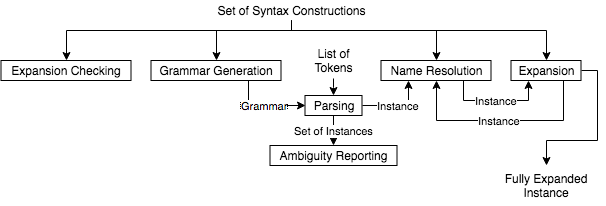
\includegraphics[width=\textwidth]{resources/formalization-flowchart}
\caption{The different algorithms that formalize syntax constructions, and how they relate to each other.}
\label{fig:formalization-flowchart}
\end{figure}

For the purposes of this section the system as a whole takes two inputs:

\begin{description}
  \item[A list of tokens] The source code we wish to parse and process, represented as a list of tokens.
  \item[A set of syntax constructions] All the syntax constructions that may be used throughout the system. A subset of these specify the programming language in which the source code is written. The rest are part of the core language, or any intermediary language.
\end{description}

The final output is a fully expanded \emph{instance} of some syntax construction. For all intents and purposes, an instance is an abstract syntax tree (AST) of the source code we are processing, and the two terms will mostly be used interchangeably. ''Fully expanded'' means that it only contains constructs from the core language, all higher-level language constructs have been expanded and replaced with lower-level constructs.

Section~\ref{sec:defining-syntax-constructions} defines the various components that make up a single syntax construction, which all other sections will then use.

We will now briefly describe the different parts of Figure~\ref{fig:formalization-flowchart} and describe their relation to each other. Expansion checking can be run entirely separately from the rest of the system, but requires previous knowledge from the other parts, and will thus be explained last.

\emph{Grammar generation} (Section~\ref{sec:formalization-grammar-generation}) takes a set of syntax constructions, more precisely the set that defines our language, and produces a context-free grammar (CFG).

\emph{Parsing} (Section~\ref{sec:formalization-parsing}) takes the CFG from grammar generation and the list of tokens describing the source code and produces zero or more instances (ASTs). Zero instances means parsing failed, one means it succeeded, more than one means the source code was ambiguous.

\emph{Ambiguity reporting} (Section~\ref{sec:implementation-ambiguity-detection}) takes a set of instances and produces an error message of the form ''these parts of the source code are ambiguous'', thus being more informative than the trivial ''the source code is ambiguous''.

\emph{Name resolution} (Section~\ref{sec:name-resolution}) takes the complete set of syntax constructions and an instance, and checks the instance for binding errors. The binding semantics for an instance is specified in the syntax construction of which it is an instance. Name resolution also performs (binding preserving) renaming to ensure that each symbol occurs at most once in a binding position.

\emph{Expansion} (Section~\ref{sec:expansion-formalization}) takes an instance where each symbol appears in binding position at most once and expands a single instance somewhere in the AST. Note that the resulting instance might have a symbol in a binding position more than once, and there may be more instances that could be expanded. The general case will thus interleave expansion and name resolution until no more instances can be expanded, at which point the final, fully expanded instance has been produced.

\emph{Expansion checking} (Section~\ref{sec:expansion-checking-formalization}) examines a single syntax construction to ensure that it cannot introduce a binding error through expansion. This means that if an AST has no binding errors, then the expansion of some instance cannot introduce a new binding error, i.e., all errors can be reported in terms of the original source code.

As mentioned previously, expansion checking can be run entirely independently of the rest of the system, none of the other steps require it. In particular, expansion checking requires no source code and no other syntax constructions than the one currently being checked. However, all statements regarding the abstraction preserving nature of syntax constructions requires that each syntax construction has been checked and found correct. In practice, expansion checking should thus be performed before all other steps.

% The entire chapter also features a running example in the form of a language (Listing~\ref{lst:formal-language}) and some source code in that language (Listing~\ref{lst:formal-file}). The reader may wish to bookmark these listings, as this chapter is fairly long and they will be referred to throughout. The language implements simple arithmetic, a scoping construct, and a name binding construct. The core language used is a small, Lisp-like language, providing arithmetic, sequential composition, and a binding construct. This language can be found in Appendix~\ref{sec:formal-core}.

\section{Running Example} \label{sec:running-example}

The remainder of this chapter will feature a running example: a programming language (defined in Listing~\ref{lst:formal-language}) and a small source code example in that language (Listing~\ref{lst:formal-file}). The reader may wish to bookmark these listings, as this chapter is fairly long and they will be referred to throughout. This section will explain the example in greater detail.

\afterpage{
\clearpage
\newgeometry{headsep=10mm,footskip=0mm,bottom=0mm}
\begin{listing}[t!]
\inputminted[linenos]{syncon}{implementation/languages/formalization-example/language}
\caption{The language that will be used as a running example.\label{lst:formal-language}}
\end{listing}

\begin{listing}[H]
\inputminted[linenos]{text}{implementation/languages/formalization-example/file}
\caption{Source code for the running example. Should evaluate to $10$.\label{lst:formal-file}}
\end{listing}
\restoregeometry
\clearpage
}

The language consists of six syntax constructions: \syncon{top}, \syncon{var}, \syncon{lit}, \syncon{sum}, \syncon{def}, and \syncon{block}, and one syntax type: \syncon{Expression}. The language is implemented in terms of a Lisp-like core language (which can be found in Appendix~\ref{sec:formal-core}, also defined using syntax constructions).

Line 1 of Listing~\ref{lst:formal-language} defines the syntax type \syncon{Expression}, and states that its representation is the same as that of the syntax type \syncon{Core}, which is provided by the core language. We do this, instead of just using \syncon{Core} directly, for parsing reasons: when we attempt to parse an \syncon{Expression} we will only try to parse syntax constructions explicitly defined to have syntax type \syncon{Expression}. This means that our new language is syntactically separated from the core language.

The remainder of Listing~\ref{lst:formal-language} defines the six syntax constructions. As an example, consider \syncon{sum}, defined on lines~8-14. Broadly speaking, a syntax construction is defined in three parts: a \emph{header} (line~8), a \emph{syntax description} (line~9), and a \emph{body} (lines~10-14):

\begin{description}
  \item[Header:] The header declares the name of the syntax construction (\syncon{sum}) and its syntax type (\syncon{Expression}).
  \item[Syntax description:] The syntax description describes the concrete syntax of the syntax construction, i.e., how it should be parsed when we parse source code in our language.
  \item[Body:] The body is split in two parts:
  \begin{itemize}
    \item Some optional extra information, e.g., precedence (line 11), binding information (in \syncon{def}, on line 18), or scoping information (in \syncon{block}, on line 25).
    \item An expansion template (line 13), specifying how this syntax construction is to be expanded.
  \end{itemize}
\end{description}

The beginning of line 13, \syncon{Core`}, specifies that what follows should be parsed as a syntax construction of syntax type \syncon{Core}. Had it instead said \syncon{Expression`} then the remainder of the body would have been parsed as a syntax construction of syntax type \syncon{Expression}. Both would be valid when considering the syntax type of the expansion, as it only needs to be representationally equal to \syncon{Expression}. In general, parsing uses nominal syntax types while expansion uses representational syntax types. These serve as parallels to nominal and structural type systems, where the former treats differently named types as different types, while the latter treats all types with the same structure as the same type.

The remainder of line 13 is an expression in the core language, a call to the function \syncon{sum} with two arguments: \syncon{`t(a)} and \syncon{`t(b)}. These arguments represent the \syncon{Expression}s \syncon{a} and \syncon{b} from the syntax description. The ''\syncon{t}'' in \syncon{`t(a)} means that we are using a syntax construction \syncon{a}, while \syncon{`int(i)} (e.g., in \syncon{lit} on line 7) instead means that we are using an integer from the syntax description. This extra syntax for using elements from the syntax description in the expansion template is due to a limitation in the parser, and is discussed in more detail in the previous chapter, in Section~\ref{sec:design-implementation}.

The syntax description of \syncon{block}, on line~23, demonstrates an additional capability: repetitions via ''\syncon{*}''. Syntax constructions additionally support ''\syncon{+}'', and ''\syncon{?}'', as commonly seen in regular expressions and EBNF. The ''\syncon{*}'' after the parentheses on line~23 denote that a \syncon{block} can contain zero or more \syncon{Expression}s, each followed by a semicolon.

The expansion template, on lines 25-28, must then reduce the unknown number of \syncon{Expression}s to a exactly one. This is done through a left fold, folding over \syncon{es} and naming the accumulator \syncon{prev}.

Line 27 contains an expansion template, and is essentially the function we are folding with. Here \syncon{prev} will refer to the accumulator, and \syncon{es} will refer to the \emph{current} element of the list we are folding over. \syncon{seq} is sequential composition, defined in the core language, i.e., it evaluates its first argument and then returns the second.

Line 28 contains the initial value of the accumulator: an expression that will evaluate to \syncon{0}. This means that an empty \syncon{block} evaluates to zero, but otherwise has no effect, since sequential composition discards the previous value.

Three of the syntax constructions in Listing~\ref{lst:formal-language} interact with name binding: \syncon{var}, \syncon{def}, and \syncon{block}.

\syncon{var} introduces a reference to a binding. This is signified by the \syncon{Identifier} in the syntax description that does not appear in a \syncon{#bind} declaration. We say that the identifier is in a \emph{referencing position}, since it should reference a binding elsewhere. This is similar to a free identifier, as commonly used in the literature, but makes no statement on whether the identifier appears bound or free.

\syncon{def} introduces a binding \emph{after} itself, as signified by the \syncon{#bind id after} declaration on line 18. We say that this identifier is in a \emph{binding position}, since it is used to introduce a new binding. In particular, the binding is not available in \syncon{e}, this syntax construction does not allow recursive definitions. Had there been an additional declaration of the form \syncon{#bind id in e}, then recursive definitions would have been allowed.

\syncon{block} introduces a \emph{scope}, preventing bindings inside the \syncon{block} from being available outside. This is declared through \syncon{#scope (es)} on line~23, which means ''introduce a new scope that covers all repetitions of \syncon{es}.''

And finally, \syncon{File} is a syntax type introduced by the core language to represent an entire file. When parsing source code the parser will try to parse a syntax construction with this syntax type to cover the entire file. In grammar terms, \syncon{File} is the start symbol.

\section{Defining Syntax Constructions} \label{sec:defining-syntax-constructions}

This section will introduce the various components that make up a single syntax construction, finally stating the complete definition of a syntax construction at the end of the section.

Some parts of this formalization will use a line above an expression to mean a sequence of expressions. For example, $\overline{i}$ denotes a sequence of $i$s, $i_n$ denotes the $n$th element in the sequence, and $\overline{i_n + 1}$ denotes a sequence of $i_n + 1$ for each $n$ (i.e., a mapping over the sequence). For example, given the sequence $\overline{i} = [1, 2, 3]$, we have $\overline{i_n + 1} = [2, 3, 4]$. Additionally, given two sequences $\overline{a} = [1, 2]$ and $\overline{b} = [3, 4]$, $\overline{(\overline{a}, b_n)} = [([1, 2], 3), ([1, 2], 4)]$, i.e., $\overline{a}$ stays a sequence since it has no index and retains the line. An empty sequence will be written $\epsilon$.

Additionally, as is common in functional programming languages, we will use $\_$ to denote a wildcard, a something whose value is unimportant or is allowed to have any value. For example, $f(\_) = 4$ is a function that ignores its argument and always produces $4$.

\subsubsection{Syntax Type}

A syntax type $t$ is given by a name, drawn from the set of all possible syntax type names. We will write them like the syntax types in Listing~\ref{lst:formal-language}, e.g., \syncon{Expression}, \syncon{Core}, and \syncon{File}.

Line~1 in Listing~\ref{lst:formal-language} introduces the syntax type \syncon{Expression}, and additionally defines it to have the same representation as \syncon{Core}. We write:

$$
\syncon{Expression} \approx \syncon{Core}
$$

We further define $\approx$ to be reflexive, symmetric, and transitive.

For our example language all syntax constructions have the syntax type \syncon{Expression}, except \syncon{top} which has syntax type \syncon{File}.

The core language defines the syntax type \syncon{Core} as follows:

\begin{minted}{syncon}
syntax type Core = builtin
\end{minted}

This declaration only introduces the new syntax type, it does not declare it to have the same representation as any other syntax type.

Additionally, syntax type declarations must refer to previously declared syntax types. This means that each partition formed by $\approx$ has exactly one syntax type declared as \syncon{builtin}.

\subsubsection{Syntax Description}

A \emph{syntax description} describes the concrete syntax of the syntax construction it belongs to. It is defined by the following grammar:

\newcommand{\ident}{\mathrel{\mathbf{identifier}}}
\newcommand{\integer}{\mathrel{\mathbf{integer}}}
\newcommand{\float}{\mathrel{\mathbf{float}}}
\newcommand{\seq}{\mathrel{\mathbf{seq}}}
\newcommand{\repstar}{\mathrel{\mathbf{star}}}
\newcommand{\repplus}{\mathrel{\mathbf{plus}}}
\newcommand{\repquestion}{\mathrel{\mathbf{question}}}

\setlength{\grammarindent}{3em}
\begin{sgrammar}
<d> ::= $\ident$
  \alt $\mathbf{string}$
  \alt $\integer$
  \alt $\float$
  \alt \synt{token}
  \alt \ssynt{t}
  \alt $\seq$ $\overline{\ssynt{d}}$
  \alt $\repstar \ssynt{d}$
  \alt $\repplus \ssynt{d}$
  \alt $\repquestion \ssynt{d}$
\end{sgrammar}

Note that although the syntax of a syntax description is an abstract syntax, it describes a concrete syntax, and will thus contain tokens. For the remainder of this chapter, tokens will be written quoted and with a different font. For example, \syncon{"foo"} is an identifier token, while \syncon{"4"} is an integer token.

The first four alternatives of the grammar match any token of the correct type, e.g., $\integer$ will match any integer token. \synt{token} represents any literal used in the syntax description, for example \syncon{"+"} on line 9 in Listing~\ref{lst:formal-language}. These will match a token containing precisely that text, a single plus symbol in the example. $\seq$ represents a parenthesized sequence (e.g., on line~23 in Listing~\ref{lst:formal-language}), while $\repstar$, $\repplus$, and $\repquestion$ represent ''\syncon{*}'', ''\syncon{+}'', and ''\syncon{?}'', respectively.

For example, $\ssynt{d}_{\syncon{block}})$, the syntax description of \mintinline{syncon}{block} (line~23 in Listing~\ref{lst:formal-language}), is given by:

$$
\seq \syncon|"{"|\ (\repstar (\seq \syncon{Expression}\ \syncon{";"}))\ \syncon|"}"|
$$

Since the syntax used in Section~\ref{sec:design-syntax} allows multiple direct children (i.e., without using an extra set of parentheses), but the syntax above does not, we implicitly insert $\seq$ around the description to get an equivalent description.

Another notable difference between the syntax descriptions in Listing~\ref{lst:formal-language} and \ssynt{d} is that of names. The names appearing in the syntax descriptions in Listing~\ref{lst:formal-language} do not appear in the syntax description in the formalization, they are instead reintroduced in a different form later in this section.

From here we define the concept of a leaf of a syntax construction, those descendants that appear atomic: the first six alternatives in the grammar above are leaves.

\subsubsection{Syntax Construction Instance} \label{sec:defining-instances}

We will now define an \emph{instance} of a syntax construction. When the parser determines that some source code should be parsed as a syntax construction $c$, we create an instance of it. These are technically not part of the definition of a syntax description, but later concepts require knowledge of the structure of an instance.

An instance \ssynt{i} is defined by the following grammar:

\newcommand{\repseq}{\mathrel{\mathbf{rep}}}
\newcommand{\tagged}{\mathrel{\textbf{:>}}}

\setlength{\grammarindent}{3em}
\begin{grammar}
<i> ::= $c \tagged \ssynt{i}$
  \alt \synt{token}
  \alt $\seq$ $\overline{\synt{inner}}$
  \alt $\repseq$ $\overline{\synt{inner}}$
\end{grammar}

The alternatives of \ssynt{i} each represent, in order:
\begin{itemize}
  \item An instance, parsed from a syntax type \ssynt{t}. In particular, an instance of a syntax construction $c$ always has the form $c \tagged i$, meaning that $i$ is an instance of $c$.
  \item A single token, parsed from one of the first five alternatives in \ssynt{s}.
  \item A sequence, parsed from a $\seq$.
  \item A repetition, parsed from any of the three last alternatives in \ssynt{s} (i.e., the EBNF operators).
\end{itemize}

For example, the \mintinline{syncon}{block} on lines~3-6 of Listing~\ref{lst:formal-file} has the following instance:

$$
\begin{array}{l}
\syncon{block} \tagged \\
\quad \seq \syncon|"{"|\\
\quad \hphantom{\seq}\ (\repseq (\seq (\syncon{def} \tagged \ldots)\ \syncon{";"}) \\
\quad \hphantom{\seq (\repseq}\ (\seq (\syncon{lit} \tagged \ldots)\ \syncon{";"})) \\
\quad \hphantom{\seq }\ \syncon|"}"| \\
\end{array}
$$

where $\syncon{def} \tagged \ldots$ is the instance of the \mintinline{syncon}{def} on line~3, and $\syncon{lit} \tagged \ldots$ is the instance of the \syncon{lit} on line~4.

As a parallel to the leaves of a syntax construction, we define the leaves of an instance to be the \synt{token}s and \synt{instance}s that are reachable without passing through some other \synt{instance}. The leaves of the \syncon{block} instance above are the curly braces, the semi-colons, the $\syncon{def} \tagged \ldots$, and the $\syncon{lit} \tagged \ldots$.

\newcommand{\leaves}{\ensuremath{\mathit{leaves}}}

More concretely, we compute the set of leaves of an instance using \leaves:

\newcommand{\children}{\ensuremath{\mathit{children}}}
$$
\begin{array}{rcl}
\leaves(c \tagged i) & = & \children(i) \\
\children(\synt{token}) & = & \{\synt{token}\} \\
\children(c \tagged i) & = & \{c \tagged i\} \\
\children(\seq \overline{i}) & = & \bigcup_n \children(i_n) \\
\children(\repseq \overline{i}) & = & \bigcup_n \children(i_n) \\
\end{array}
$$
\let\children\undefined

These will be useful in later sections (e.g. name resolution) that deal with leaves, the instance to which they belong, and the syntax construction the instance was instantiated from.

\subsubsection{Paths}

We will now reintroduce the names used in the syntax descriptions of Listing~\ref{lst:formal-language}. Each name will be replaced by a path, a series of steps traversing \ssynt{d} or \ssynt{i}, selecting the element(s) to which the name referred. The specific formulation used below allow the same path to be used both in a syntax description and an instance, and additionally provide a simple way to refer to specific repetitions (from EBNF operators), a concept that is important for name resolution and expansion.

A path is given by the following grammar:

\setlength{\grammarindent}{3em}
\begin{sgrammar}
<p> ::= $n : p$
\alt $* : p$
\alt $[]$
\end{sgrammar}

Where $n$ is a positive number. We will additionally write $[a, b, c]$ as shorthand for $a : b : c : []$. Informally, a step $n$ traverses through the $n$th child, while a step $*$ traverses through \emph{all} children. We will generally use $p$ to range over paths, and $P$ to range over sets of paths.

Each path belongs to some syntax construction $c$, and should only be used for traversal in the syntax description of $c$, or an instance of $c$. This is equivalent to saying that a name referring to an element of the syntax description of $c$ is only meaningful for $c$.

\newcommand{\follow}{\mathit{follow}}

For traversal, we define a function $\follow$. This function allows us access to the element(s) the names referred to, and once we introduce more operations for manipulating paths, access to specific subsets of what the names referred to. To traverse \ssynt{d}:

$$
\begin{array}{rcl}
\follow([], i) &=& i \\
\follow(n : p, \seq \overline{i}) &=& \follow(p, i_n) \\
\follow(\_ : p, \repstar i) &=& \follow(p, i) \\
\follow(\_ : p, \repplus i) &=& \follow(p, i) \\
\follow(\_ : p, \repquestion i) &=& \follow(p, i) \\
\end{array}
$$

Note that we only allow a $*$ to step through one of the EBNF operators, $\follow(* : p, \seq \overline{i})$ is not defined. To traverse \ssynt{i}:

$$
\begin{array}{rcl}
\follow([], i) &=& \{i\} \\
\follow(n : p, \seq \overline{i}) &=& \follow(p, i_n) \\
\follow(n : p, \repseq \overline{i}) &=& \follow(p, i_n) \\
\follow(* : p, \repseq \overline{i}) &=& \bigcup_n \follow(p, i_n) \\
\end{array}
$$

As a consequence on the limitation on $*$, a traversal in \ssynt{d} produces a single element, while traversal in \ssynt{i} produces a (possibly empty) set of elements.

Translating a name to a path is now a matter of finding the corresponding node $d'$ in the syntax description $d$, and producing a path $p$ such that $\follow(p, d) = d'$, and every traversal through one of $\repstar$, $\repplus$, or $\repquestion$ is done using a $*$. For example, the syntax description of \syncon{block} (on line~23 in Listing~\ref{lst:formal-language}) has the following form:

$$
\seq \syncon|"{"|\ (\repstar (\seq \syncon{Expression}\ \syncon{";"}))\ \syncon|"}"|
$$

The name \syncon{es} (also on line~23) refers to the \syncon{Expression}. We find that \syncon{Expression} appears in the second element of the outer $\seq$, inside the $\repstar$ expression, in the first element of the inner $\seq$. The path $[2, *, 1]$ describes this traversal, i.e., $\follow(2, *, 1], d) = \syncon{Expression}$.

The \syncon{block} instance on lines~3-6 in Listing~\ref{lst:formal-file} has the following form:

$$
\begin{array}{l}
\syncon{block} \tagged i =
\syncon{block} \tagged \\
\hphantom{\syncon{block} \tagged i =}\ \quad \seq \syncon|"{"|\\
\hphantom{\syncon{block} \tagged i =}\ \quad \hphantom{\seq}\ (\repseq (\seq (\syncon{def} \tagged \ldots)\ \syncon{";"}) \\
\hphantom{\syncon{block} \tagged i =}\ \quad \hphantom{\seq (\repseq}\ (\seq (\syncon{lit} \tagged \ldots)\ \syncon{";"})) \\
\hphantom{\syncon{block} \tagged i =}\ \quad \hphantom{\seq }\ \syncon|"}"| \\
\end{array}
$$

We thus find that $\follow([2, *, 1], i) = \{(\syncon{def} \tagged \ldots), (\syncon{lit} \tagged \ldots)\}$. If we wished to only access the first repetition of \syncon{es}, we could in stead use the path $[2, 1, 1]$: $\follow([2, 1, 1], i) = \{(\syncon{def} \tagged \ldots)\}$

\subsubsection{Scope}

\newcommand{\near}{\ensuremath{\mathrel{\mathbf{near}}}}
\newcommand{\scope}{\ensuremath{\mathrel{\mathbf{scope}}}}

A \emph{scope} introduces a limit on where a binding introduced by \syncon{#bind before} or \syncon{#bind after}: no binding introduced inside a scope is available outside of it. It is given by the following grammar:

\setlength{\grammarindent}{3em}
\begin{sgrammar}
<s> ::= $\scope$ $p$ $P$ $\ssynt{s}$
  \alt $\near$
\end{sgrammar}

where $p$ is a path and $P$ is a set of paths. The first alternative represents a scope introduced via a \syncon{#scope} declaration (e.g., line~25 in Listing~\ref{lst:formal-language}). $p$ describes how often the scope repeats (i.e. \syncon{#scope repeat:(...)}), while $P$ contains paths to the leaves included in the scope (i.e. \syncon{#scope (leaf1 leaf2)}). The final component is the parent scope.

The second alternative is the special scope $\near$, which is the ancestor scope of all other scopes. It represents the scope to which the syntax construction instance belongs, i.e., the nearest surrounding scope.

Note that, similar to paths, each scope belongs to a single syntax construction. They will not be discussed without a clear connection to a syntax construction or instance.

\newcommand{\cover}{\ensuremath{\mathit{cover}}}
We also introduce the concept of \cover: the cover of a scope is a set of paths to the leaves it contains:

% MARK: TODO: continue here
$$
\begin{array}{rcl}
\cover(\scope \_\ P \_) & = & P \\
\cover(\near) & = & \{\text{The leaves not covered by another scope}\} \\
\end{array}
$$

We require that all leaves are covered by some scope, defaulting to $\near$ if no other scope applies. Additionally, no two scopes may cover the same leaf. To create nesting scopes we instead create parent-child connections between two scopes.

For example, \syncon{block} in Listing~\ref{lst:formal-language} has two scopes: \near\ and $(\scope []\ \{[2, *, 1]\} \near)$. Their covers are $\{[1], [2, *, 2], [3]\}$ and $\{[2, *, 1]\}$, respectively. The latter scope corresponds to the \syncon{#scope (es)} declaration on line~25, thus the cover is a single path to \syncon{es}. \near\ then covers everything else, in this case the curly braces and the semicolon.

\subsubsection{Expansion Template}

An \emph{expansion template} describes how the expansion of a particular syntax construction should be created. It is essentially an instance with holes, which are filled using elements from the instance being expanded or folds over elements from the instance being expanded. An expansion template is given by the following grammar:

\newcommand{\acc}{\mathrel{\mathbf{acc}}}
\newcommand{\foldl}{\mathrel{\mathbf{foldl}}}

\setlength{\grammarindent}{3em}
\begin{sgrammar}
<e> ::= $p$
  \alt $\acc n$
  \alt $\foldl p$ \ssynt{e} \ssynt{e}
  \alt $c \tagged \ssynt{i_e}$

<i_e> ::= <token>
  \alt \ssynt{e}
  \alt $\seq \overline{\ssynt{i_e}}$
  \alt $\repseq \overline{\ssynt{i_e}}$
\end{sgrammar}

The $\acc n$ alternative refers to the accumulator of a surrounding fold, the innermost if $n = 0$, second inner-most if $n = 1$, etc. This is essentially a de bruijn index, except instead of a lambda binding an argument, we have a fold binding an accumulator. The actual implementation additionally has a right fold, as well as $\mathit{fold1}$ variations of both, where the first element of the list is used as the initial value of the accumulator while folding over the tail of the list, but these are omitted here for brevity.

The \mintinline{syncon}{block} syntax construction in Listing~\ref{lst:formal-language} has the following expansion template (lines~26-28):

$$
\begin{array}{l}
\foldl [2, *, 1] \\
\quad \syncon{coreseq} \tagged (\seq \syncon{"("}\ \syncon{"seq"}\ (\acc 0)\ [2, *, 1]\ \syncon{")"}) \\
\quad \syncon{corelit} \tagged (\seq \syncon{"0"}) \\
\end{array}
$$

\syncon{coreseq} and \syncon{corelit} are defined in the core language mentioned in the description of the running example, in Section~\ref{sec:running-example}. This definition can be found in Appendix~\ref{sec:formal-core}.

An additional point here is that of recursion: many macro systems allow a macro to expand to code containing the macro itself, but syntax constructions do not (neither directly nor indirectly). Disallowing recursion loses some expressive power, however, we contend that EBNF operators and folds mostly make up for this loss in practice, and we gain some nice termination guarantees instead. This will be discussed further in Section~\ref{sec:expansion-formalization}.

\subsubsection{Precedence and Associativity}

The precedence of a syntax construction is a number or $+\infty$. The former represents a syntax construction that has a defined precedence (e.g., \syncon{sum}, via \syncon{#prec 2} on line~11 in Listing~\ref{lst:formal-language}), while the latter represents a syntax construction without a defined precedence (e.g., \syncon{var}, defined on lines~4-5 in Listing~\ref{lst:formal-language}).

Associativity is represented by one of three values:

\begin{sgrammar}
<a> ::= \textbf{left} | \textbf{right} | \textbf{none}
\end{sgrammar}

\textbf{left} and \textbf{right} represent left and right associativity, while \textbf{none} represents undefined associativity.

\subsubsection{Syntax Construction}

Putting it all together, a syntax construction $c$ is given by a tuple
$$ c = (t_c, d_c, S_c, B_n, B_b, B_a, p_c, a_c, e_c) $$
with the following components:

\begin{tabular}{r|p{10cm}}
$t_c$ & The syntax type of $c$ \\
$d_c$ & The syntax description of $c$ \\
$S$ & The scopes introduced by $c$, a set of scopes. \\
$B_n$ & The nested bindings of $c$, a set of tuples $(p, P)$ where the first element is a path to an identifier and the second is a set of paths to the leaves where it is in scope. \\
$B_b$ and $B_a$ & The bindings $c$ exports before and after itself, respectively. Sets of paths to identifiers. \\
$p_c$ & The precedence of $c$, $+\infty$ unless otherwise specified. \\
$a_c$ & The associativity of $c$. \\
$e_c$ & The expansion template of $c$. \\
\end{tabular}

A 9-tuple is somewhat unwieldy, thus later sections will generally refer to ''the $B_n$ of $c$'' to refer to the nested bindings of $c$, etc., instead of listing the entire tuple and picking out the relevant component. The components that appear with $c$ in their subscript are exceptions to this, e.g., $t_c$ refers to the syntax type of $c$.

As an example, the syntax construction \syncon{block}, defined on lines~22-29 of Listing~\ref{lst:formal-language} has the following form:

$$
(t_{\syncon{block}}, d_{\syncon{block}}, S_{\syncon{block}}, B_n, B_b, B_a, p_{\syncon{block}}, a_{\syncon{block}}, e_{\syncon{block}})
$$
where
$$
\begin{array}{rcl}
t_{\syncon{block}} &=&
\syncon{Expression}
\\

d_{\syncon{block}} &=&
\seq \syncon|"{"|\ (\repstar (\seq \syncon{Expression}\ \syncon{";"}))\ \syncon|"}"|
\\

S_{\syncon{block}} &=&
\{\near, \scope []\ \{[2, *, 1]\} \near\}
\\

B_n &=& \emptyset
\\

B_b &=& \emptyset
\\

B_a &=& \emptyset
\\

p_{\syncon{block}} &=& +\infty
\\

a_{\syncon{block}} &=& \textbf{none}
\\

e_{\syncon{block}} &=&
\foldl [2, *, 1] \\
& & \quad \syncon{coreseq} \tagged (\seq \syncon{"("}\ \syncon{"seq"}\ (\acc 0)\ [2, *, 1]\ \syncon{")"}) \\
& & \quad \syncon{corelit} \tagged (\seq \syncon{"0"}) \\
\end{array}
$$

From this we also define our concept of a language: a language defined using syntax constructions is a set of syntax constructions.

\section{Source Code Parsing}

The diagram in Figure~\ref{fig:formalization-flowchart} contains three components that are relevant to parsing code written in a language defined using syntax constructions: Grammar Generation, Parsing, and Ambiguity Reporting. This section will describe them, along with their connections to each other.

\subsection{Grammar Generation} \label{sec:formalization-grammar-generation}

The algorithm for translating a set of syntax constructions to a context-free grammar proceeds as described below, using the following notation:

\mathligsoff
{\tabulinesep=2mm
\begin{tabu}{c|p{10cm}}
$N^t_p$ & A non-terminal generated by the constructions $c$ such that $t = t_c \land p = p_c$. \\
$next(N^t_p)$ & The non-terminal with the next higher precedence. \\
$N^t_-$ & Shorthand for the non-terminal generated by the lowest precedence group in $t$. \\
$N^t_+$ & Highest precedence group in $t$. Note that $N^t_+ \neq N^t_-$ is not true in general, some syntax types only contain syntax constructions of a single precedence level. \\
\end{tabu}
}

\begin{enumerate}
  \item Group syntax constructions by their syntax type, then by precedence.
  \item For each such group, generate a non-terminal $N^t_p$:
  \begin{itemize}
    \item For each syntax construction $c$, generate one production according to its syntax description:
    \begin{itemize}
      \item $\ident$, $\integer$, $\float$, and $\mathbf{string}$ each match one token of the corresponding kind.
      \begin{itemize}
        \item $\ident$ should not match an identifier with a symbol that is used as a literal in any syntax construction.
      \end{itemize}
      \item A token literal matches a token with exactly the same contents.
      \item References to a syntax type $t'$ matches non-terminals according to the following, picking the first that applies:
      \begin{itemize}
        \item If $t \neq t'$, match $N^{t'}_-$.
        \item If $c$ has the highest precedence in $t$, match $N^t_-$.
        \item If $c$ has undefined associativity, or is left-associative and $t'$ is the leftmost occurrence, or is right-associative and $t'$ is the rightmost occurrence, match $N^t_{p_c}$.
        \item Otherwise match $next(N^t_{p_c})$.
      \end{itemize}
      \item A $\seq$ matches each of its children in turn.
      \item EBNF operators ($\repstar$, $\repplus$, and $\repquestion$) match repetitions as expected.
    \end{itemize}
  \end{itemize}
  \item For each non-terminal $N^t_i$ except $N^t_+$ add a production matching the non-terminal $next(N^t_i)$.
\end{enumerate}
\mathligson

For our example language, grouping by syntax type and then precedence gives the following grouping:

\begin{itemize}
  \item \mintinline{syncon}{File}
  \begin{description}
    \item[$+\infty$] \mintinline{syncon}{top}
  \end{description}

  \item \mintinline{syncon}{Expression}
  \begin{description}
    \item[$1$] \mintinline{syncon}{def}
    \item[$2$] \mintinline{syncon}{sum}
    \item[$+\infty$] \mintinline{syncon}{var}, \mintinline{syncon}{lit}, and \mintinline{syncon}{block}
  \end{description}
\end{itemize}

Generating production rules according to point 2 gives the following grammar:

\setlength{\grammarindent}{9em}
\begin{grammar}
<FileInf> ::= <Expression1>

<Expression1> ::= 'def' <Identifier> '=' <Expression1>

<Expression2> ::= <Expression2> '+' <ExpressionInf>

<ExpressionInf> ::= <Identifier>
  \alt <Integer>
  \alt '$\{$' (<Expression1> ';')* '$\}$'
\end{grammar}

where \synt{Identifier} will not match an identifier that is exactly \syncon{"def"}.

Note how the three \mintinline{syncon}{Expression}s refer to each other: \synt{Expression1} only references itself, \synt{Expression2} references itself and \synt{ExpressionInf}, and \synt{ExpressionInf} only references \synt{Expression1}. These references are determined by the precedence and associativity of the syntax construction that generated each production.

This grammar is not particularly useful however, since neither \synt{Expression2} nor \synt{ExpressionInf} are reachable from the start symbol \synt{FileInf}. Step 3 solves this by introducing an extra production to each of \synt{Expression1} and \synt{Expression2}, which produces our final grammar:

\setlength{\grammarindent}{9em}
\begin{grammar}
<FileInf> ::= <Expression1>

<Expression1> ::= 'def' <Identifier> '=' <Expression1>
  \alt <Expression2>

<Expression2> ::= <Expression2> '+' <ExpressionInf>
  \alt <ExpressionInf>

<ExpressionInf> ::= <Identifier>
  \alt <Integer>
  \alt '$\{$' (<Expression1> ';')* '$\}$'
\end{grammar}

\subsection{Parsing} \label{sec:formalization-parsing}

We here assume the presence of a parsing algorithm that can handle an arbitrary context-free grammar, for example the Earley \cite{Earley1970An-Efficient-Co} parsing algorithm. In particular, if the source code cannot be parsed unambiguously then we must be able to construct all possible parse trees.

With this in mind, the inputs of this step are the following:

\begin{itemize}
  \item A context-free grammar produced by the previous section.
  \item A token stream representing the source code to be parsed.
\end{itemize}

The output then has three possible forms:

\begin{itemize}
  \item A single parse tree, from which we produce an instance. This is the successful case. We proceed to the next step, Name Resolution, in Section~\ref{sec:name-resolution}.
  \item No parse trees, we could not parse the source. This is the simple failure case, report an error to the user.
  \item Two or more parse trees, from which we produce one instance each. This is the ambiguous case, the more complex failure case, in which case we move on to the next section, Ambiguity Reporting.
\end{itemize}

\subsection{Ambiguity Reporting} \label{sec:implementation-ambiguity-detection}

If the parse step produced multiple instances we have encountered source code that was ambiguous, i.e., it could be parsed in multiple ways. We could trivially report to the user that the code is ambiguous and that they must clarify their intent, but merely stating that an entire file is ambiguous provides very little assistance in locating the problem.

Instead we wish to produce an error that refers only to the actually ambiguous parts of the source file. Furthermore, we wish to present the different parse trees in an understandable way.

Starting with the second point, assume that no operators have defined precedence or associativity and consider the following expression:

$$ a + b * c $$

It can be parsed in two ways:

$$ (a + b) * c $$
$$ a + (b * c) $$

The former is a product of a sum and a variable, the latter is a sum of a variable and a product. Further describing the inner structure of the sub-expressions (sum of two variables and product of two variables respectively), gives little to no extra useful information for understanding the two parsings. Consider this more complicated example:

$$ a + b + c + d $$

The parsings are as follows:

$$ ((a + b) + c) + d $$
$$ (a + (b + c)) + d $$
$$ (a + b) + (c + d) $$
$$ a + ((b + c) + d) $$
$$ a + (b + (c + d)) $$

All of these are sums, the first two of a sum and a variable, the next of two sums, the last two of a variable and a sum. This form of description, i.e., a single top-level node and a shallow description of its children, will be referred to as a two-level representation.

As an example, consider the following code:

\begin{minted}{text}
1 + 2 + 3
\end{minted}

Parsing this code using the running example language (Listing~\ref{lst:formal-language}), but without associativity for \mintinline{syncon}{sum}, we obtain the following two instances:

$$
\begin{array}{l|l}
\begin{array}{l}
\syncon{top} \tagged (\seq \\
\quad \syncon{sum} \tagged (\seq \\
\qquad (\syncon{sum} \tagged \\
\qquad \quad \seq (\syncon{lit} \tagged\ \seq \syncon{"1"}) \\
\qquad \quad \hphantom{\seq}\ \syncon{"+"} \\
\qquad \quad \hphantom{\seq}\ (\syncon{lit} \tagged\ \seq \syncon{"2"})) \\
\qquad \syncon{"+"} \\
\qquad (\syncon{lit} \tagged\ \seq \syncon{"3"}))) \\
\end{array}
&
\begin{array}{l}
\syncon{top} \tagged (\seq \\
\quad \syncon{sum} \tagged (\seq \\
\qquad \syncon{"+"} \\
\qquad (\syncon{lit} \tagged\ \seq \syncon{"1"}) \\
\qquad (\syncon{sum} \tagged \\
\qquad \quad \seq (\syncon{lit} \tagged\ \seq \syncon{"2"}) \\
\qquad \quad \hphantom{\seq}\ \syncon{"+"} \\
\qquad \quad \hphantom{\seq}\ (\syncon{lit} \tagged\ \seq \syncon{"3"})))) \\
\end{array}
\end{array}
$$

Replacing these with two-level representations of the actual ambiguity gives us the following:

\begin{itemize}
  \item A \mintinline{syncon}{sum} of a \mintinline{syncon}{sum} and a \mintinline{syncon}{lit}.
  \item A \mintinline{syncon}{sum} of a \mintinline{syncon}{lit} and a \mintinline{syncon}{sum}.
\end{itemize}

There is an additional subtlety in what we wish to consider as a two-level representation, stemming from the presence of internal structure in the form of $\seq$ and $\repseq$. In the example above we only consider full instances, not the internal structure, but we could just as well have chosen the following two-level representations:

\begin{itemize}
  \item A $\seq$ of a \mintinline{syncon}{sum} and a \mintinline{syncon}{lit}.
  \item A $\seq$ of a \mintinline{syncon}{lit} and a \mintinline{syncon}{sum}.
\end{itemize}

This choice is discussed in more detail in the evaluation, in Section~\ref{sec:errors-ambiguous}. The remainder of this section will assume the second alternative (i.e., use $\seq$ and $\repseq$) and leave the first alternative as a potential engineering decision.

The task of producing an error message then becomes selecting subtrees from the syntax trees such that:

\begin{itemize}
  \item The unselected parts are identical across the different syntax trees, including covered source area (i.e., we report all ambiguities).
  \item The selected subtrees from the same position across the syntax trees cover the same source area (i.e., each report has a clear connection to the source).
  \item At least two selected subtrees in the same position of their respective syntax tree have different two-level representations (i.e., all reports actually show different parsings).
  \item No selected subtree is contained in another (i.e., we only report one ambiguity per source file area).
  \item No selected subtree can be replaced by one of its children (also replacing the corresponding subtrees from the other syntax trees) while still satisfying the points above (i.e., the selected subtrees are minimal).
\end{itemize}

To accomplish this, we use a form of shallow equality where two nodes are equal if they cover the same source area and have the same kind (e.g., they are instances of the same syntax construction). With this in mind we traverse all the syntax trees in parallel, top to bottom, until we encounter a node that is shallowly different between at least two syntax trees. If any sibling of the node also is shallowly different, select the parent, otherwise select the node and keep traversing down the siblings.

Finally, present to the user a set of two-level representations for each selected subtree across the syntax trees.

% TODO: it is not actually obvious that the algorithm satisfies all the requirements above, nor that all requirements are required, nor that it's always possible to satisfy all requirements.

% it satisfies covers same area (because difference in area would mean start and end point are different, i.e. one of the versions covers a token the other does not, but then that token must be covered by a sibling, or a sibling of the parent, etc., in which case the sibling is shallowly different, or the parent is shallowly different, etc.)
% it satisfies no overlap (trivial)
% it satisfies minimal (only select something shallowly equal if multiple children are shallowly different, i.e. would need to replace by multiple subtrees)
% it satisfies shows difference (trivial)
% it satisfies report all (trivial)

% TODO: the minimal requirement is a bit weirdly formulated, we might rephrase it as (no [...] can be replaced by one or more of its children [...]), but then we need to check especially for coverage differences, so if any of the children have coverage differences across the ASTs then we select the parent, otherwise we select the children

As an example, consider our running example, but once again with associativity removed for \syncon{sum}. Since Listing~\ref{lst:formal-file} contains \syncon{a + 2 + 3} we know that parsing it will produce multiple instances, in this case two. In the interest of brevity we will only show two levels of the instances at once, the node currently being compared and its children, but not its grandchildren. We will denote shallow equality by $=_s$. Stepping through the ambiguity reporting we start by examining the top-level node of the respective trees:

$$
\begin{array}{rcl}
\syncon{top} \tagged (\seq \ldots)
& =_s &
\syncon{top} \tagged (\seq \ldots) \\
\end{array}
$$

$$
\begin{array}{rcl}
\seq (\syncon{block} \tagged \ldots)
& =_s &
\seq (\syncon{block} \tagged \ldots) \\
\end{array}
$$

$$
\begin{array}{rcl}
\syncon{block} \tagged (\seq \ldots)
& =_s &
\syncon{block} \tagged (\seq \ldots) \\
\end{array}
$$

$$
\begin{array}{rcl}
\seq \syncon|"{"|\ (\repseq \ldots)\ \syncon|"}"|
& =_s &
\seq \syncon|"{"|\ (\repseq \ldots)\ \syncon|"}"| \\
\end{array}
$$

$$
\begin{array}{rcl}
\syncon|"{"| & =_s & \syncon|"{"| \\

\repseq (\seq \ldots)\ (\seq \ldots)
& =_s &
\repseq (\seq \ldots)\ (\seq \ldots) \\

\syncon|"}"| & =_s & \syncon|"}"| \\
\end{array}
$$

$$
\begin{array}{rcl}
\seq (\syncon{def} \tagged \ldots)\ \syncon{";"}
& =_s &
\seq (\syncon{def} \tagged \ldots)\ \syncon{";"} \\

\seq (\syncon{sum} \tagged \ldots)\ \syncon{";"}
& =_s &
\seq (\syncon{sum} \tagged \ldots)\ \syncon{";"} \\
\end{array}
$$

Under normal circumstances we would now have to descend into both children (i.e., both $(\seq \syncon{def} \ldots)$ and $(\seq \syncon{sum} \ldots)$), but in the interest of brevity we will instead note that the first child is fully equal across the two trees (there is no ambiguity there). Descending through it will thus never come across any instances that are not shallowly equal. We will thus only concern ourselves with descent into the second child:

$$
\begin{array}{rcl}
\syncon{sum} \tagged (\seq \ldots)
& =_s &
\syncon{sum} \tagged (\seq \ldots) \\

\syncon{";"} & =_s & \syncon{";"} \\
\end{array}
$$

$$
\begin{array}{rcl}
\seq (\syncon{sum} \tagged \ldots)\ \syncon{"+"}\ (\syncon{lit} \tagged \ldots)
& =_s &
\seq (\syncon{var} \tagged \ldots)\ \syncon{"+"}\ (\syncon{sum} \tagged \ldots)
\end{array}
$$

This is the first point where we see any inequality, but the two instances are still shallowly equal, since both have the form $(\seq \ldots)$ and both cover the same area of the source code.

$$
\begin{array}{rcl}
\syncon{sum} \tagged (\seq \ldots)
& \not=_s &
\syncon{var} \tagged (\seq \ldots) \\

\syncon{"+"} & \not=_s & \syncon{"+"} \\

\syncon{lit} \tagged (\seq \ldots)
& \not=_s &
\syncon{sum} \tagged (\seq \ldots) \\
\end{array}
$$

Note here than none of the children are shallowly equal. In particular, the \syncon{"+"} tokens cover different areas of the source code (they are the second and first ''\syncon{+}'' in the source code respectively). We thus select the parent and present that as the one ambiguity in the source code.

\section{Further Properties of Paths} \label{sec:paths}

This section will introduce further path-related concepts that will be used in the later sections.

As a reminder, a path allows a syntax construction to refer to its children through a traversal. Each step of the traversal is either an index $n$ that traverses down the child at index $n$, or a $*$ traversing through \emph{all} children. We write the empty path $[]$, prepending $n$ to a path $p$ as $n : p$, and use $[a, b, c]$ as shorthand for $a : b : c : []$.

We now define a relation $p_1 \subseteq p_2$ between two paths, where

$$
\begin{array}{ll}
p \subseteq p & (\subseteq \text{is reflexive}) \\
n : p \subseteq n : p' & \text{ if } p \subseteq p' \\
n : p \subseteq * : p' & \text{ if } p \subseteq p' \\
\end{array}
$$

% TODO: the \forall here is a little bit iffy, since we only consider things for a single syntax construction
We justify the notation by noting that given two paths $p_1$ and $p_2$ that belong to syntax construction $c$, and that $s$ is the syntax description of $c$, we have:

$$
\begin{array}{rcl}
p_1 \subseteq p_2 & -> & \follow(p_1, s) = \follow(p_2, s) \\
p_1 \subseteq p_2 & -> & \forall (c \tagged i).\ \follow(p_1, i) \subseteq \follow(p_2, i) \\
\end{array}
$$

We see this by noting that the structure of an instance mirrors that of the syntax description, and that a $*$ step is only allowed through an EBNF operator (i.e., $\repstar$, $\repplus$, or $\repquestion$ in the syntax description, and $\repseq$ in an instance). We say that $p_1$ is a more specific version of $p_2$.

For example, $[2, 1, 1] \subseteq [2, *, 1]$. The former selects the first sub-expression in a \mintinline{syncon}{block} instance (Listing~\ref{lst:formal-language}), while the latter selects \emph{all} sub-expressions.

\newcommand{\specialize}{\ensuremath{\mathit{specialize}}}

We also wish to be able to specialize a path $p$ using some other path $p'$, i.e., $\specialize(p, p') \subseteq p$. Note that the fourth case below allow $p$ and $p'$ to diverge (i.e., we do not require $p' \subseteq p$), in which case the specialization is only applied to their shared prefix.

$$
\begin{array}{rcl}
\specialize(p, []) & = & p \\
\specialize(*:p, n:p') & = & n : \specialize(p, p') \\
\specialize(*:p, *:p') & = & * : \specialize(p, p') \\
\specialize(n:p, n':p') & = &
\begin{cases}
  p & n \neq n' \\
  n : \specialize(p, p') & n = n' \\
\end{cases} \\
\end{array}
$$

For example, $\specialize([2, *, 2, *], [2, 1, 1, 1]) = [2, 1, 2, *]$.

\section{Name Resolution} \label{sec:name-resolution}

\newcommand{\rooti}{\ensuremath{\mathit{root}}}

Name resolution is a structure and binding preserving transformation that replaces each symbol in an abstract syntax tree with newly generated ones so as to ensure that each symbol appears in a binding position at most once across the entire tree. Additionally, name resolution detects the presence of binding errors. The root of the tree will be referred to as \rooti, and will by construction have the shape $c \tagged i$ (i.e., it is an instance of some syntax construction $c$).

We assume that each node is unique and distinct from all other nodes in the tree, and in particular that it can be used as the key in a mapping. This could, for example, be accomplished by attaching a unique number to each node across the tree. Furthermore, we can attach an ordering between two nodes if neither is a descendant of the other. A node $a$ is before another node $b$ if it appears earlier in the tree, in which case we will write $a < b$.

% TODO: is "to the left" sufficiently well defined?

This section will also be strict about the distinction between an identifier and a symbol: an identifier is a node in the syntax tree, and it contains a symbol. As an example,

\begin{minted}{text}
{
  def a = 1;
  def a = 2;
}
\end{minted}

\newcommand{\sym}{\ensuremath{\mathit{symbol}}}
\newcommand{\symlit}[1]{\text{''#1''}}

has two identifiers with the same symbol: \symlit{a}. We will write $\sym(i)$ to denote the symbol of the identifier $i$. A symbol will be written as its text in quotations, i.e., \symlit{a} is a symbol, not to be confused with \syncon{"a"}, which is an identifier.

First, we wish to find all the identifiers that are in a binding position:

\newcommand{\binders}{\ensuremath{\mathit{binders}}}

$$
\begin{array}{rcl}
\binders(c \tagged i) & = & i_b \cup i_a \cup i_n \cup i_c \\
\text{where} & & \\
i_b & = & \{ \follow(p, i) \mid p \in B_b \text{ of } c\} \\
i_a & = & \{ \follow(p, i) \mid p \in B_a \text{ of } c\} \\
i_n & = & \{ \follow(p, i) \mid (p, \_) \in B_n \text{ of } c\} \\
i_c & = & \bigcup_{(c' \tagged i') \in \leaves(c \tagged i)} \binders(c' \tagged i') \\
\end{array}
$$

For example, using the instance for the innermost \mintinline{syncon}{block} (writing it as $\syncon{block} \tagged i$) in Listing~\ref{lst:formal-file}:

$$
\begin{array}{rcl}
\binders(\syncon{block} \tagged i) & = & i_b \cup i_a \cup i_i \cup i_c = \{\syncon{"a"}\}\\
\text{where} & & \\
i_b & = & \{ \follow(p, i) \mid p \in \emptyset \} = \emptyset \\
i_a & = & \{ \follow(p, i) \mid p \in \emptyset \} = \emptyset \\
i_i & = & \{ \follow(p, i) \mid (p, \_) \in \emptyset \} = \emptyset \\
i_c & = & \binders(\syncon{def} \tagged \ldots) = \{\syncon{"a"}\} \\
\end{array}
$$

Second, we need a mapping $\Gamma$ from $\binders(\rooti)$ to new unique symbols. The particular details of this mapping are unimportant, we merely require it to map different nodes to different symbols.

Third, we wish to determine the scope of each node in the tree. Similar to syntax constructions and their instances we introduce scope instances, described by the following grammar:

\newcommand{\rootscope}{\ensuremath{\mathrel{\text{\textbf{root-scope}}}}}
\newcommand{\scopeinst}{\mathrel{\text{\textbf{scope-inst}}}}

\begin{grammar}
<scope-instance> ::= $\scopeinst P$ <scope-instance>
  \alt \rootscope
\end{grammar}

The first case represents most instances and consists of two components: a set of paths to the leaves it covers, and its parent scope instance. The second case is the root scope.

For example, the outermost \mintinline{syncon}{block} instance in Listing~\ref{lst:formal-file} (lines~1-7) introduces one scope instance:

$$
(\{[2, *, 1]\}, \rootscope)
$$

We will further write $s'_c -> s'_p$ to mean that $s'_p$ is the parent scope of $s'_c$, and $s' ->* s''$ as the reflexive, transitive closure of this relation. Since each node will be assigned to a single scope we will write $i \in s'$ to mean that $i$ belongs to scope instance $s'$, which then selects a unique scope instance per $i$.

Additionally, we will define the scope instance of $\rooti$ to be $\rootscope$, i.e.:

$$ \rooti \in\ \rootscope $$

\newcommand{\instantiate}{\ensuremath{\mathit{instantiate}}}

Given a scope $s$ and a path $p$ to a leaf, both belonging to an instance $c \tagged i$, the scope instance of $s$ is given by $\instantiate(c \tagged i, p, s)$:

$$
\begin{array}{rcl}
\instantiate(c \tagged i, p, \near) & = & s' \text{ where } c \tagged i \in s' \\
\instantiate(c \tagged i, p, \text{(}rep, P, s\text{)}) & = & \text{(}P', parent\text{)} \\
\instantiate(c \tagged i, p, \scope r\ P\ s) & = & \scopeinst P'\ s' \\
\text{where} & & \\
r' & = & \specialize(r, p) \\
P' & = & \{\specialize(p', r') \mid p' \in P\} \\
s' & = & \instantiate(c \tagged i, p, s) \\
\end{array}
$$

We are now ready to determine the scope instance any non-root leaf belongs to. Given a leaf $i$, that is a leaf of $c \tagged i'$, find the scope $s$ in $c$ that covers $i$, then instantiate it:

$$
\inference{
  i \in \leaves(c \tagged i') &
  follow(p, i') = \{i\} &
  p \subseteq p' \\
  p' \in \cover(s) &
  s \in scopes \text{ of } c
}{i \in \instantiate(c \tagged i', p, s)}
$$

We can now start considering actual bindings. For each node we will compute a set of available bound symbols. Each binding is represented by a 3-tuple consisting of a symbol, a scope instance, and a generated symbol. The first two components denote that the symbol definition is in the given scope instance, while the last component is the generated replacement symbol from $\Gamma$ above.

As an example, $\{(\symlit{foo}, s'_1, \symlit{bar}), (\symlit{foo}, s'_2, \symlit{baz})\}$ has two bindings of the symbol $\symlit{foo}$, one bound in $s'_1$, the other in $s'_2$, replaced by $\symlit{bar}$ and $\symlit{baz}$ respectively.

\newcommand{\lookup}{\ensuremath{\mathit{lookup}}}

The $\lookup$ function below defines shadowing behavior: a binding of a symbol in a child scope shadows the same symbol in a parent scope. The first case also assumes that we will never produce a binding set with more than one element that share the first two components, which would represent a redefinition of a symbol in the same scope.

$$
\lookup(\mathit{sym}, s', \gamma) =
\begin{cases}
\mathit{sym}' & (\mathit{sym}, s', \mathit{sym}') \in \gamma \\
\lookup(\mathit{sym}, s'', \gamma) & (\mathit{sym}, s', \_) \not\in \gamma \land s' -> s'' \\
\bot & (\mathit{sym}, s', \_) \not\in \gamma \land s' =\ \rootscope
\end{cases}
$$

At this point we have our definitions for binding errors: an unbound symbol produces $\bot$ during lookup, while a redefinition produces a binding set where two or more elements share the first two components.

The latter error has some subtleties. We could defer the error until $\lookup$ would find multiple choices, i.e., make it an error to have an ambiguous reference instead of making it an error to redefine a symbol, but the latter tends to be a programming error even if it does not lead to any ambiguity.

The exported \syncon{before} and \syncon{after} bindings of an instance $(c \tagged i) \in s'$, written as $E_b(c \tagged i)$ and $E_a(c \tagged i)$ respectively, are given by:

$$
\begin{array}{rcl}
E_b(c \tagged i) & = & \mathit{immediate} \cup \mathit{transitive} \\
\text{where} & & \\
\mathit{transitive} & = & \bigcup_{(c' \tagged i') \in \leaves(c \tagged i), (c' \tagged i') \in s'} E_b(c' \tagged i') \\
\mathit{immediate} & = & \bigcup_{p \in B_b} \{(\sym(\follow(p, i)), s', \Gamma(\follow(p, i)))\}
\end{array}
$$

$$
\begin{array}{rcl}
E_a(c \tagged i) & = & \mathit{immediate} \cup \mathit{transitive} \\
\text{where} & & \\
\mathit{transitive} & = & \bigcup_{(c' \tagged i') \in \leaves(c \tagged i), (c' \tagged i') \in s'} E_a(c' \tagged i') \\
\mathit{immediate} & = & \bigcup_{p \in B_a} \{(\sym(\follow(p, i)), s', \Gamma(\follow(p, i)))\}
\end{array}
$$

Bindings can also be defined in a nested manner, via $B_n$. The bindings visible in a node $i \in \leaves(c \tagged i')$ where $follow(p, i') = \{i\}$, is given by $E_n(i)$:

$$
\begin{array}{rcl}
E_n(\rooti) & = & \emptyset \\
E_n(i) & = & E_n(c \tagged i'\})\ \cup \\
& & \{ symbol(\follow(p, i')) \mid (p, P) \in B_n \land \exists p' \in P.\ p \subseteq p'\} \\
\end{array}
$$

Note the difference between $E_a(i)$, $E_b(i)$, and $E_n(i)$: the former two give the set of bindings \emph{exported} by $i$, while the latter gives the set of bindings \emph{usable} in $i$.

% TODO: MARK: I've gotten this far in the formalization "rewrite", everything beyond this point has only been update to be consistent in syntax (i.e. c~i vs c\{i\} vs (c \tagged i))

With all this setup, name resolution is a matter of replacing the symbol in each identifier that was parsed from $\ident$ (as opposed to a token literal) with a newly generated symbol. Given an identifier $id \in \leaves(c \tagged i)$ with scope $id \in s'$, $\follow(p, i) = \{id\}$, and $syntax$ being the syntax description of $c$, we will only perform the below substitution if $\follow(p, syntax) =\ \ident$.

$$
\begin{array}{rcl}
\sym(id) & <- &
\begin{cases}
\Gamma(id) & id \in \binders(\rooti) \\
\lookup(\sym(id), s', \gamma) & id \not\in \binders(\rooti) \\
\end{cases} \\
\text{where} & & \\
\gamma & = & a \cup b \cup E_n(id) \\
a & = & \bigcup_{(c' \tagged i') \in s'' \land s' ->* s'' \land (c' \tagged i') < id} E_a(c' \tagged i') \\
b & = & \bigcup_{(c' \tagged i') \in s'' \land s' ->* s'' \land (c' \tagged i') > id} E_b(c' \tagged i') \\
\end{array}
$$

\section{Expansion} \label{sec:expansion-formalization}

Expanding the instance of a syntax construction is relatively straightforward, but the formalization turns out to be surprisingly involved. The base idea is that an expansion is a template into which we splice subtrees from the instance we are expanding, similar to pattern based macros in Lisp tradition. As an additional precondition we assume that the symbols present in the initial instance only occur in binding position at most once.

The process is made somewhat more complicated by the presence of EBNF operators that generate lists, which must be reduced to a single subtree through folds. To perform such a fold we require specific paths to each of the elements to be folded over, to be handed to $\specialize$ later:

\newcommand{\specs}{\ensuremath{\mathit{specs}}}

$$
\begin{array}{rcl}
\specs([], i) & = & \{[]\} \\
\specs(n:p, \seq \overline{i}) & = & \{n : p' \mid p' \in \specs(p, i_n)\} \\
\specs(n:p, \repseq \overline{i}) & = & \{n : p' \mid p' \in \specs(p, i_n)\} \\
\specs(*:p, \repseq \overline{i}) & = & \bigcup\limits_{n} \{n:p' \mid p' \in \specs(p, i_n)\} \\
\end{array}
$$

Note that while this function uses set-notation, the order of the paths will be important while folding. The order is easily recovered however using a simple lexicographic sorting of the paths. All later uses of $\specs$ will thus be considered to return an ordered sequence of paths, rather than a set.

As an example, consider the outermost \mintinline{syncon}{block} instance (covering all lines) obtained from the code in Listing~\ref{lst:formal-file}. It has the following form:

$$
\begin{array}{l}
\syncon{block} \tagged \\
\quad \seq \syncon|"{"|\\
\quad \hphantom{\seq}\ (\repseq (\seq (\syncon{def} \tagged \ldots)\ \syncon{";"}) \\
\quad \hphantom{\seq (\repseq}\ (\seq (\syncon{sum} \tagged \ldots)\ \syncon{";"})) \\
\quad \hphantom{\seq }\ \syncon|"}"| \\
\end{array}
$$

As such $\specs([2, *, 1], \syncon{block} \tagged \ldots) = [[2, 1, 1] [2, 2, 1]]$.

\newcommand{\expand}{\ensuremath{\mathit{expand}}}

Expansion (via $\expand$ below) then traverses the template (the fourth argument, $e_c$), while keeping track of the current item in a fold ($p$), the related accumulators ($\overline{acc}$), and the instance being expanded ($i$). Most cases are fairly straightforward recursion:

$$
\begin{array}{rcl}
\expand(i, p, \overline{acc}, p') & = & i' \text{ where } \follow(\specialize(p', p), i) = \{i'\} \\
\expand(i, p, \overline{acc}, \acc~n) & = & acc_n \\
\expand(i, p, \overline{acc}, c \tagged i') & = & c \tagged \expand(i, p, \overline{acc}, i') \\
\expand(i, p, \overline{acc}, \synt{token}) & = & \synt{token} \\
\expand(i, p, \overline{acc}, \seq \overline{i'} ) & = & \seq \overline{\expand(i, p, \overline{acc}, i'_n)} \\
\expand(i, p, \overline{acc}, \repseq \overline{i'}) & = & \repseq \overline{\expand(i, p, \overline{acc}, i'_n)} \\
\end{array}
$$
The one remaining case, $\foldl$, is somewhat more involved:
$$
\begin{array}{rcl}
\expand(i, p, \overline{acc}, \foldl~p'~f~i') & = & \mathit{foldl}(f', f_0, P) \\
\end{array}
$$
where
$$
\begin{array}{rcl}
f' & = & \lambda p'~acc'.~ \expand(i, p', acc'~\overline{acc}, f) \\
f_0 & = & \expand(i, p, \overline{acc}, i') \\
P & = & \specs(\specialize(p', p), inst) \\
\end{array}
$$

and $\mathit{foldl}$ is a regular left fold over a list.

As an example, \syncon{block} has the following expansion template:

$$
\begin{array}{l}
\foldl [2, *, 1] \\
\quad \syncon{coreseq} \tagged (\seq \syncon{"("}\ \syncon{"seq"}\ (\acc 0)\ [2, *, 1]\ \syncon{")"}) \\
\quad \syncon{corelit} \tagged (\seq \syncon{"0"}) \\
\end{array}
$$

Expanding the instance given above proceeds as follows, using $i$ to refer to that instance:

$$
\begin{array}{l}
\expand(i, [], \epsilon, \foldl~[2, *, 1]~(\syncon{coreseq} \tagged \ldots)~(\syncon{corelit} \tagged \ldots)) \\
\qquad = \mathit{foldl}(f', f_0, P) \\
\end{array}
$$
where
$$
\begin{array}{rcl}
f' & = & \lambda p'~acc'.~ \expand(i, p', [acc'], \syncon{corelit} \tagged \ldots) \\
f_0 & = & \expand(i, [], \epsilon, \syncon{corelit} \tagged (\seq \syncon{"0"}) \\
& = & \syncon{corelit} \tagged \expand(i, [], \epsilon, \seq \syncon{"0"}) \\
& = & \syncon{corelit} \tagged (\seq \expand(i, [], \epsilon, \syncon{"0"})) \\
& = & \syncon{corelit} \tagged (\seq \syncon{"0"}) \\
P & = & \specs(\specialize([2, *, 1], []), i) \\
& = & \specs([2, *, 1], i) \\
& = & [[2, 1, 1], [2, 2, 1]] \\
\end{array}
$$

$\mathit{foldl}$ will then call $f'$ twice, once with $p' = [2, 1, 1]$ and $acc' = f_0$, and once with $p' = [2, 2, 1]$ and $acc' = f_1$, where $f_1$ is the result of the previous call. It is here useful to note that a subtree that does not contain either $\acc~n$ or a path always expands to itself, hence we will omit those expansions below.

The first $f'$ call proceeds as follows:

$$
\begin{array}{rcl}
f'~[2, 1, 1]~f_0 & = & \expand(i, [2, 1, 1], f_0, \syncon{coreseq} \tagged (\seq \ldots)) \\
& = & \syncon{coreseq} \tagged \\
& & \quad \expand(i, [2, 1, 1], f_0, \seq \\
& & \qquad \syncon{"("} \\
& & \qquad \syncon{"seq"} \\
& & \qquad \acc~0 \\
& & \qquad [2, *, 1] \\
& & \qquad \syncon{")"}) \\
& = & \syncon{coreseq} \tagged \\
& & \quad \seq \\
& & \qquad \syncon{"("} \\
& & \qquad \syncon{"seq"} \\
& & \qquad \expand(i, [2, 1, 1], f_0, \acc~0) \\
& & \qquad \expand(i, [2, 1, 1], f_0, [2, *, 1]) \\
& & \qquad \syncon{")"} \\
& = & \syncon{coreseq} \tagged \\
& & \quad \seq \\
& & \qquad \syncon{"("} \\
& & \qquad \syncon{"seq"} \\
& & \qquad f_0 \\
& & \qquad (\syncon{def} \tagged \ldots) \text{ since} \\
& & \qquad \quad \follow(\specialize([2, *, 1], [2, 1, 1]), i) \\
& & \qquad \qquad = \follow([2, 1, 1], i) \\
& & \qquad \qquad = (\syncon{def} \tagged \ldots) \\
& & \qquad \syncon{")"} \\
& = & f_1 \\
\end{array}
$$

The second call, with the identical steps omitted, then follows:

$$
\begin{array}{rcl}
f'~[2, 2, 1]~f_1 & = & \syncon{coreseq} \tagged \\
& & \quad \seq \\
& & \qquad \syncon{"("} \\
& & \qquad \syncon{"seq"} \\
& & \qquad \expand(i, [2, 1, 1], f_1, \acc~0) \\
& & \qquad \expand(i, [2, 1, 1], f_1, [2, *, 1]) \\
& & \qquad \syncon{")"} \\
& = & \syncon{coreseq} \tagged \\
& & \quad \seq \\
& & \qquad \syncon{"("} \\
& & \qquad \syncon{"seq"} \\
& & \qquad f_1 \\
& & \qquad (\syncon{sum} \tagged \ldots) \text{ since} \\
& & \qquad \quad \follow(\specialize([2, *, 1], [2, 2, 1]), i) \\
& & \qquad \qquad = \follow([2, 2, 1], i) \\
& & \qquad \qquad = (\syncon{sum} \tagged \ldots) \\
& & \qquad \syncon{")"} \\
\end{array}
$$

% TODO: this is not the most understandable justification, to say the least. there is a part of an alternate explanation below it
At this point we can consider termination guarantees: the expansion of a single syntax construction instance must terminate. We see this easily from the definition of $\expand$ and the observation that the expansion template is finite. Furthermore, since syntax constructions may not recursively expand into instances of themselves (neither directly nor indirectly), the complete expansion of a syntax tree must also terminate. We can see this by noting that when we expand an instance of a syntax construction $c$ then none of the instances introduced by the expansion (i.e., not the ones copied over from the previous instance) are instances of $c$, nor can they expand into instances of $c$. To expand those instances we thus never need $c$, i.e., the number of syntax constructions required for expansion is reduced by one. Since the number of syntax construction is finite we will eventually reach a point where we cannot expand any further since no remaining syntax construction has an expansion, i.e., the syntax tree is fully expanded.

% We can see this by forming a directed acyclic graph where there is an edge from a syntax construction to another if the first might expand to a syntax tree containing the other, then sorting the syntax constructions in topological order. If we then expand all occurrences of the first syntax construction (call it $c$) the resulting syntax tree contains no instances of $c$, nor can an instance of $c$ occur from further expansion of other syntax construction. Expanding the second syntax construction similarly removes it, etc., until

\section{Expansion Checking} \label{sec:expansion-checking-formalization}

Expansion checking extends name resolution to handle special 'placeholder' nodes, nodes that represent instances of syntax constructions, and that conceptually reference all symbols in scope and export one symbol \mintinline{syncon}{before}, one \mintinline{syncon}{after}, and one in both.

By definition, for a placeholder node $p \in s'$ we have

$$ binders(p) = \{p_e, p_b, p_a\} $$
$$ E_b(p) = \{(\sym(p_e), s', \Gamma(p_e)), (\sym(p_b), s', \Gamma(p_b))\} $$
$$ E_a(p) = \{(\sym(p_e), s', \Gamma(p_e)), (\sym(p_a), s', \Gamma(p_a))\} $$

where $p_e$, $p_b$, and $p_a$ are unique identifiers with unique symbols. Additionally we will consider the computed set of bindings in scope (i.e., $\gamma$ in the previous section) for a placeholder node $p$, but without the replacement symbols, to be an output of name resolution, which we will refer to as $\gamma_p$.

The idea here is that no actual instance will have greater requirements on its surroundings than a placeholder node, thus if expanding an instance where all children are placeholders introduces no errors, then expanding the same instance but with actual instances should also not introduce errors.

More concretely, given a syntax construction instance $c \tagged i$ where all identifiers have different symbols and all child instances are in fact placeholders, and its expansion $e = \expand(i, [], \epsilon, e_c)$, then an error might be introduced if one of the following is true:

\begin{enumerate}
  \item There is a placeholder $p'$ somewhere in $e$, copied from a placeholder $p$ in $c \tagged i$, such that $\gamma_p \setminus \gamma_{p'} \neq \emptyset$ (i.e., $p$ might reference a symbol before expansion that $p'$ cannot afterwards).
  \item $E_b(e) \setminus E_b(c \tagged i) \neq \emptyset$ or $E_a(e) \setminus E_a(c \tagged i) \neq \emptyset$ (i.e., the instance might export something before expansion, but not after).
  \item Any symbol in an identifier in a referencing position in $e$ that is unbound is \emph{bound} in an identifier in a referencing position in $c \tagged i$.
\end{enumerate}

The third point warrants further elaboration. The checking procedure examines an instance in isolation, i.e., it is not a subtree of some syntax tree. This means that any identifier that appears in a referencing position is unbound, which is an error. However, if the same instance appeared in a syntax tree and that tree had no binding errors, then all those identifiers must be bound in that context. Replacing the instance with its expansion and placing it in the same context then satisfies the same references in the expansion. A new unbound error with a new symbol would not have this guarantee and might thus introduce an error where there were none before.

Checking the expansion definition of a syntax construction then becomes a matter of generating a representative set of instances with placeholders that cover all possible real instances that could appear in a real syntax tree. In the absence of EBNF operators this is a single instance, since no variation is possible without picking different child instances, but in their presence more care must be taken.

A 'zero or one' repetition ($\repquestion$) clearly requires two variations, but the unbounded repetitions ($\repstar$ and $\repplus$) are less clear.

A fold over a $\repstar$ repetition could result in the initial accumulator value only, or one or more iterations of the actual folding template. The folding template can only use the accumulator atomically, so it will essentially wrap it in some other expression, possibly copied in multiple places. It is the hypothesis of this thesis that errors can occur either when fold and initial value interact, or when a fold interacts with a previous fold, and that no such interaction requires multiple folds to appear, because of the limited capabilities of each fold. If this holds true then all possible errors should appear by simply checking 0, 1, and 2 repetitions. Similarly, a $\repplus$ repetition could be used in a $\mathit{fold1}$ fold which would require 3 repetitions to exhibit two wrapped applications of the fold template.

\newcommand{\gen}{\mathit{gen}}
\newcommand{\genrep}{\mathit{rep}}

% TODO: this is a pretty bad explanation. maybe I can actually use a monad? :(

The $\gen$ function, given below, generates the necessary variations. Note that it is not written as a pure function, the first two cases should generate new unique results every time they are called. Also note that the third case ($\seq$) and $\genrep$ should be considered to generate one variation per choice of variation from the sets generated by their children, basically a set cross-product. The nodes of a syntax description that do not interact with name binding can be largely ignored, except that something must be in their place in the instance (\textbf{dummy} below), otherwise the instance would be malformed, and paths would not be correct.

% TODO: is case three (sequence) clear in what it means? (all possible combinations choosing one from the variations of each item in the sequence) (essentially crossproduct of all the respective sets)

$$
\begin{array}{rcl}
\gen(\ident) & = & \mathit{uniqueId} \\
\gen(\synt{syntax-type}) & = & \mathit{uniquePlaceholder} \\
\gen(\seq \overline{syntax}) & = & \{\seq \overline{\gen(syntax_n)}\} \\
\gen(\repstar syntax) & = & \bigcup_{n=0}^2 \genrep(syntax, n) \\
\gen(\repplus syntax) & = & \bigcup_{n=1}^3 \genrep(syntax, n) \\
\gen(\repquestion syntax) & = & \bigcup_{n=0}^1 \genrep(syntax, n) \\
\gen(\_) & = & \{\textbf{dummy}\} \\
\text{where} & & \\
\genrep(syntax, n) & = & \{(\repseq \gen(syntax)\ldots)\} \\
& & \text{(Generate $n$ repetitions of $syntax$)} \\
\end{array}
$$

Nested repetitions incur many more variations as we wish to be sure to capture all possible error interactions. For example, two consecutive $\repstar$ repetitions produce $3 * 3 = 9$ variations, while two nested $\repstar$ repetitions produce $1 + 3 + 3*3 = 12$ variations.

% TODO: we make no mention here or elsewhere about how to check that the syntax types agree during expansion. Presumably this is easy to do, basically compare to the syntax description and check that repr(type-in-syntax) = repr(type-in-instance) for every expansion in the expansion checking phase

\chapter{Evaluation} \label{sec:evaluation}

The evaluation of this thesis is largely empirical and based on case studies facilitated by a proof of concept implementation of the descriptions in the previous section, along with a small interpreter for a core language. An overview of this implementation is given in Section~\ref{sec:implementation}.

The actual evaluation consists of case studies of expressibility (Section~\ref{sec:case-studies}), reuse of language feature from one language in another (Section~\ref{sec:language-composition}), a brief examination of the correctness of the implementations in the case studies (Section~\ref{sec:correctness-and-performance}), a few performance metrics of the implementation (Section~\ref{sec:performance}), and finally an examination of the errors presented to a user when something goes wrong (Section~\ref{sec:error-reporting}).

For evaluation, two programming languages have been implemented: a subset of Lua\footnote{https://www.lua.org/} and a subset of OCaml\footnote{https://ocaml.org/}. The former evaluates the expressibility of a relatively standard untyped, imperative language, while the latter evaluates the expressibility of  a relatively standard functional language, with an extra focus on pattern matching. Note that the implementation of the OCaml subset does not have static type checking, following the delimitations in Section~\ref{sec:delimitations}.

For each of the languages, a few interesting features are discussed, including their implementation, along with several limitations of the system.

\section{Implementation} \label{sec:implementation}

\begin{figure}[t]
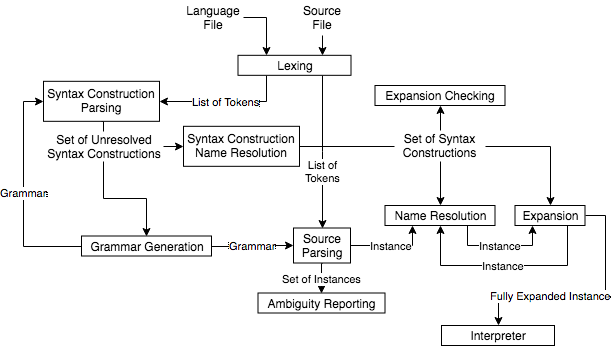
\includegraphics[width=\textwidth]{resources/implementation-flowchart}
\caption{The components that make up the implementation, and their connections}
\label{fig:implementation-flowchart}
\end{figure}

This section contains a high level overview of the proof of concept implementation of the ideas in this thesis.

The implementation is written in Haskell and is available on GitHub\footnote{https://github.com/elegios/master-thesis}. It is structured similarly to compiler with multiple phases. The phases, represented as boxes in Figure~\ref{fig:implementation-flowchart}, are as follows:

\begin{description}
  \item[Lexing] The lexer is intended to be the simplest possible lexer that still produces results suitable for the grammars later generated by the syntax constructions. It lexes everything as identifiers, symbols, or string, integer or float literals. Most adjacent punctuation and special characters are merged into single symbols, with a few exceptions to create behavior similar to other programming languages. For example, parentheses will never merge, thus \mintinline{c}{(a++)} will lex as \mintinline{syncon}{symbol('(')}, \mintinline{syncon}{identifier('a')}, \mintinline{syncon}{symbol('++')} and \mintinline{syncon}{symbol(')')}.

  \item[Syntax construction parser] The syntax construction parser is a simple context-free grammar, parsed using an Earley \cite{Earley1970An-Efficient-Co} parser. It is somewhat complicated by the need to parse arbitrary source code in the expansion template. This is solved by merging the syntax construction grammar with the generated grammar from grammar generation. Due to a limitation in the parser implementation used, the grammar cannot be modified during parsing, thus the expansion description of a syntax construction cannot use syntax constructions defined in the same file, only ones defined in an earlier file.

  The syntax constructions are unresolved, meaning that no names are connected to their definitions. These unresolved syntax constructions are usable for grammar generation, but the remaining phases require additional processing.

  \item[Syntax construction name resolver] The syntax construction name resolver will prepare the parsed syntax constructions for use later in the implementation. All names used are resolved to locations in the syntax description and an expansion function is produced for syntax constructions that are not marked as builtin. Note that this phase does some checking of the syntax construction, but only what is necessary to produce the binding information and expansion function. The checking here is not sufficient to ensure that no binding errors appear during expansion.

  \item[Expansion checking] The expansion checker checks that an expansion can never introduce an error during expansion. Similar to type checking and various other forms of static analysis, the expansion checker is not a necessary part, but its absence does of course remove any guarantees on errors.

  \item[Grammar generation] The grammar generator generates a context-free grammar from a set of syntax constructions and which will later be used to parse source code using an Earley \cite{Earley1970An-Efficient-Co} parser.
  \begin{description}
    \item[Ambiguity reporting] If the grammar is ambiguous, and the source code being parsed exposes this ambiguity, one parse tree will be produced for each possible parse, and all of them will be compared to determine the ambiguous sections of the source code.
  \end{description}

  \item[Name resolution] The name resolver takes a syntax tree generated by the parser and checks for name binding errors. If none are found all symbols are replaced with newly generated symbols in such a way that each symbol appears in a binding position exactly once, while preserving the referencing relation between identifiers.

  \item[Expansion] The source code expander repeatedly finds a single syntax construction to expand, expands it, then runs the name resolver over the result, until all remaining syntax constructions are marked as builtin. This is the simplest implementation that will always be correct, but it almost always does far more work than necessary. See Section~\ref{sec:performance} for more information.

  \item[Core language interpreter] The core language interpreter evaluates a syntax tree composed only of syntax constructions that are part of the core language described in Section~\ref{sec:core-language}, but is largely unrelated to syntax constructions as such. It is only used for validation in Section~\ref{sec:correctness-and-performance}.
\end{description}

\subsection{Core Language} \label{sec:core-language}

Syntax constructions does not specify a core language, but instead treats any construction marked as ''builtin'' as a core language construct, expanding all constructions encountered until only builtin constructions remain. However, to evaluate the expressibility of semantics for syntax constructions such a language must exist. This section describes the core language used throughout the evaluation section.

Both language subsets are implemented using the same underlying language, i.e., the same set of syntax constructions marked as builtin (for more information, see Section~\ref{sec:design-implementation}). The core language is a largely functional language using curried functions and eager execution, with a few additions:
\begin{itemize}
  \item Sequential composition.
  \item Non-nested bindings, i.e \mintinline{syncon}{defAfter} and \mintinline{syncon}{defAround}. % TODO: probably refer to a previous definition / explanation of this
  \item Builtin values using special syntax, such as \mintinline{syncon}{#unit}, \mintinline{syncon}{#true} and \mintinline{syncon}{#plus}. More complex features introduced via such values include:
  \begin{description}
    \item[Conditional execution] via \mintinline{syncon}{#if}.
    \item[Fixpoint operator] via \mintinline{syncon}{#fix}.
    \item[Mutable references] via \mintinline{syncon}{#ref}, \mintinline{syncon}{#deref}, and \mintinline{syncon}{#assign}.
    \item[Lists] via \mintinline{syncon}{#cons}, \mintinline{syncon}{#head}, \mintinline{syncon}{#tail}, and \mintinline{syncon}{#nil}.
    \item[Continuations] via \mintinline{syncon}{#callcc}.
  \end{description}
  \item Expression functions. Syntactically similar to a function (\mintinline{syncon}{efun x. body} vs. \mintinline{syncon}{fun x. body}) these work around a limitation in syntax constructions. They are described in more detail in the next section, but in brief: they are functions that take an expression, returns an expression, and are evaluated at compile-time.
\end{itemize}

All syntax constructions in the core language have syntax type \syncon{BExpression}.

\subsubsection{Expression Functions} \label{sec:efun-drawbacks}

Several syntax constructions in the evaluated languages turn out to require some information about their context, some examples include:

\begin{itemize}
  \item A \mintinline{lua}{return} statement must exit the surrounding function.
  \item A pattern in a pattern match needs a value to compare to.
  \item A \mintinline{lua}{break} statement must exit the surrounding loop.
\end{itemize}

The only way to connect multiple syntax constructions in their current design is through the name binding system: one construction defines a binding, another uses it. This requires user interaction however, the identifiers must be in the source code written by the user. None of the examples above follow such a pattern, they are all expected to obtain their information through their lexical context.

In some cases this can be solved through a function, for example, a pattern might expand to a function that expects the value to compare to as its argument. Problems arise when the syntax construction both requires information from its context, and additionally needs to expose bindings via \syncon{#bind before} or \syncon{#bind after}. Functions introduce a scope around their body, preventing any such bindings from being visible.

To solve this issue we extend our core language with an additional kind of function, one that takes an expression as an argument and evaluates at compile-time. Essentially an anonymous macro. An \syncon{efun} will not prevent accidental name capture, but since they are evaluated after the expansion provided by the syntax construction implementation, name resolution has already happened, i.e., all identifiers that do not relate to each other have different symbols.

For example,

\begin{minted}{syncon}
(efun a. #add a a) (#add 3 4)
// evaluates to
#add (#add 3 4) (#add 3 4)
// (at compile-time)
\end{minted}

We define the syntax construction as follows:

\begin{minted}{syncon}
syntax exprfun:BExpression =
  "efun" x:Identifier "." e:BExpression
{
  #bind x in e
  builtin
}
\end{minted}

Now we can let a pattern take the value to compare through an \syncon{efun}, and provide the bindings we need.

The problem is that the above definition is insufficient; the binding semantics are not properly described.

To demonstrate why, consider the following code:

\begin{minted}{syncon}
(efun a. defAfter x = a) x
\end{minted}

\syncon{defAfter} creates a new name binding for the remainder of the scope, but does not allow a recursive definition; we could not replace \syncon{a} with \syncon{x} in the example since it is not bound. However, the second occurrence of \syncon{x} in the example \emph{is} bound, since it occurs after the definition. Evaluating the \syncon{efun} produces the following:

\begin{minted}{syncon}
defAfter x = x
\end{minted}

The former produces no binding errors, but the latter does. Using a binding defined inside an \syncon{efun} in an argument to the same \syncon{efun} might create problems, but we have no way of expressing this restriction using syntax constructions. An expansion may thus appear to be correct to the expansion checker, since it preserves all specified binding semantics, and yet introduce a binding error when the \syncon{efun} is evaluated.

The second problem is one of inconvenience, many syntax constructions may now need to take arguments and pass them on to their children, even though they themselves have no use of them. For example, to get information from a loop to a \mintinline{lua}{break} statement it may need to be passed through many intermediate statements.

This additionally has an impact on composing multiple languages. No new syntax constructions can be added in-between the syntax construction that gives the context and the one that uses it without threading the information, but the odds of a syntax construction from a different language being written to thread the same information seem minuscule, thus importing a syntax construction from a different language is unlikely to work if either language uses that kind of contextual information.

Expression functions are thus not the ideal solution, but a better option is left for future work.

\section{Case Studies in Expressiveness} \label{sec:case-studies}

This section evaluates the expressiveness of syntax constructions through a number of cases. The first two implement subsets of two pre-existing programming languages: OCaml and Lua. The former focuses on implementing pattern matching and a fairly standard functional programming language, while the latter focuses on implementing control flow commonly present in imperative programming languages. The final section examines several smaller examples not present in either language that demonstrate limitations of syntax constructions.

% TODO: probably write about efuns and their drawbacks separately from each language below, seems weird to either duplicate it, or to just have it in one of the language sections and not the other, since they should have no dependenceies on each other

% TODO: own thoughts, to be made into actual evaluation thoughts later
% Control flow altering things are difficult to include without either explicit support for the particular control flow, or names that can be bound across constructions without appearing in the original source code. The return statement must be able to connect to the return point, without anything outside it altering it. Could be done if the construction returned a "function", that takes the return point and produces the actual expanded code, but that is not possible at present.

% - The efun builtin is unsound, but something like it is required to implement some of the things when each sub-construction is atomic
% - fix seems reasonable
% - callcc probably reasonable, but probably not necessary to have the full support, instead basically have it be a block that you can break out of by calling a function. Not entirely sure if that can be represented in a sound way with the current system
% - ocaml _ pattern and list literals are either inescapably ambiguous, or require rewritings that require knowledge of grammars (which we're trying to avoid)
% - funccall in lua requires splitting out the argument list, to ensure correct recursion (the call must have high precedence, but the argument list must reach for top level expressions)
% - binding expressibility has thus far been sufficient, nothing I've wanted to express has been impossible.
% - defAround allows for recursive definitions, which will be incorrect for most/many languages, but there is nothing that preserves that abstraction

% - (current) absence of checking probably means that at least one implementation is incorrect, only working because the implemented languages are sane when they introduce names. I suspect the general case, when any syntax type can bind in any way, is broken.

\subsection{A Functional Language - OCaml Subset} \label{sec:functional-eval}

% TODO: ref ocaml
The functional language implemented here is a subset of OCaml, with a focus on supporting pattern matching. This section will not examine the entirety of the language definition, most syntax constructions used are fairly simple and rote, focus will instead be placed on the implementation of patterns and pattern matching, as well as additional, difficult to express particulars of the language. The full language description can be found in Appendix~\ref{sec:appendix-ocaml}.

\subsubsection{Patterns and Pattern Matching} \label{sec:functional-pattern-matching}

Pattern matching is a feature found in most functional languages, allowing the programmer to simultaneously check the structure of data and extract internal data from it. Patterns describe the expected shape of the data, as well as what internal data should be extracted and bound to names for later use. They can be arbitrarily nested, allowing a simple way of expressing a potentially quite tedious checking process. Listing~\ref{lst:ocaml-match-example} shows an example of a match expression in OCaml, wherein the first match arm with a matching pattern is selected for execution.

\begin{listing}[ht]
\begin{minted}{ocaml}
let result = match [[4]] with
  | [[a], b] ->
    print_string "a:int, b:int list, both bound"
  | _ :: _ :: _ ->
    print_string "nothing bound, length >= 2"
  | [[4]] ->
    print_string "nothing bound"
  | _ ->
    print_string "nothing else matched"
\end{minted}
\caption{Example match expression in OCaml}
\label{lst:ocaml-match-example}
\end{listing}

The above suggests a fairly clear formulation of the syntax and bindings of the match expression using syntax constructions.

\begin{minted}{syncon}
syntax match:Expression =
  "match" e:Expression "with"
  arm:("|" p:Pattern "->" body:Expression)+
{
  #scope arm:(p body)
  #scope (e)
  <...>
}
\end{minted}

Patterns expose their bound names using \mintinline{syncon}{#bind x after} and each match arm introduces a new scope containing its pattern and expression. The patterns themselves are also simple to express in terms of syntax and bindings:

\begin{minted}{syncon}
syntax wildcardPattern:Pattern = "_" {
  <...>
}

syntax bindPattern:Pattern = id:Identifier {
  #bind id after
  <...>
}

syntax integerLiteralPattern:Pattern = i:Integer {
  <...>
}

syntax consPattern:Pattern =
  head:Pattern "::" tail:Pattern
{
  #assoc right
  #prec 10
  <...>
}
\end{minted}

% TODO: this needs to refer to some more thorough description / discussion of the lexer and its choices

Implementing each of these is where problems arise; each pattern must do two things:

\begin{itemize}
  \item Check a value provided by the enclosing pattern or match expression. The result of this check must be usable to change control flow.
  \item Possibly expose a bound name, where the bound value is derived from the checked value, but only needs to be valid if the check succeeded.
\end{itemize}

The former implies a function, each pattern might be implemented as a function receiving the value to check and producing a boolean value signifying the result of the check. The latter precludes the use of a function, since a function introduces a new scope, thus preventing any bound name from being available outside its body.

Other pattern match systems implemented as macros (e.g., \cite{Tobin-Hochstadt2011Extensible-Patt}) tend to have a more complicated match macro, which constructs the final checking code and binding code by examining the actual contents and / or results of the patterns. Syntax constructions on the other hand have no such functionality, child nodes may only be treated atomically, i.e., moved, removed, or duplicated. As such the composing mechanism must be present in the pattern implementation, but it cannot be a function, since it would hide name bindings.

For example, the following definition of \syncon{bindPattern} has an incorrect expansion template; the binding introduced is hidden inside the function:

\begin{minted}{syncon}
syntax bindPattern:Pattern = id:Identifier {
  #bind id after
  BExpression` fun value.
    defAfter `id(id) = value
}
\end{minted}

As discussed in Section~\ref{sec:efun-drawbacks} we will instead use \syncon{efun}s, essentially anonymous macros.

A pattern then becomes an \syncon{efun} taking a function to call if the match fails and a value to match against. Implementation becomes as follows:

\begin{minted}{syncon}
syntax wildcardPattern:Pattern = "_" {
  BExpression` efun fail. efun value.
    #unit
}

syntax bindPattern:Pattern = id:Identifier {
  #bind id after
  BExpression` efun fail. efun value.
    defAfter `id(id) = value
}

syntax integerLiteralPattern:Pattern = i:Integer {
  BExpression` efun fail. efun value.
    #if (#equal value `int(i))
      (fun _. #unit)
      (fun _. fail #unit())
}

syntax consPattern:Pattern =
  head:Pattern "::" tail:Pattern
{
  #assoc right
  #prec 10
  BExpression` efun fail. efun value.
    (#if (#equal value #nil)
       (fun _. fail #unit)
       (fun _. #unit);
     defAfter headValue = #head value;
     `t(head) fail headValue;
     defAfter tailValue = #tail value;
     `t(tail) fail tailValue)
}
\end{minted}

The pattern implementing matching against a list literal (i.e., \mintinline{ocaml}{[a, b]} as opposed to \mintinline{ocaml}{a :: b :: []}) is a straightforward extension of the cons pattern.

Continuing, the implementation of \mintinline{ocaml}{match}, while not trivial, is a relatively straightforward composition of its match arms. For each arm, give the pattern the value to check, and a function to call to skip to checking the next arm in case the pattern fails, then evaluate the body and return the result. The implementation uses \mintinline{syncon}{callcc} to make an abortable function: \mintinline{syncon}{#callcc (fun abort. body)} evaluates to one of two things: the argument provided to \mintinline{syncon}{abort}, or the result of evaluating \mintinline{syncon}{body} if \mintinline{syncon}{abort} is never called.

\begin{minted}{syncon}
syntax match:Expression =
  "match" e:Expression "with"
  arm:("|" p:Pattern "->" body:Expression)+
{
  #scope arm:(p body)
  #scope (e)
  #prec 1
  BExpression` #callcc (fun end. (fun val.
    `t(foldr arm prev
         (BExpression`
           #callcc (fun next.
             (`t(p) next val;
              end `t(body)));
           `t(prev))
       (BExpression` #crash)))
    `t(e))
}
\end{minted}

Note that the implementation is somewhat naive, for example no work is shared between the arms, even if there is overlap in the patterns, and there are no warnings for overlapping patterns or incomplete coverage.

The syntax descriptions and binding specifications on the other hand are clear an concise and may be considered a success.

\subsubsection{Patterns in Function Declarations}
\label{sec:ocaml-function-argument-patterns}

Patterns are not limited only to the \mintinline{ocaml}{match} expression in OCaml, they can additionally be used in function definitions. The most common way of writing such a function uses \mintinline{ocaml}{let} with some syntax sugar to allow writing all the arguments next to the function name, instead of as part of nested \mintinline{ocaml}{fun} expressions. The two definitions below are equivalent, and we would like our OCaml subset to support both:

\begin{minted}{ocaml}
let add a b = a + b
let add = fun a -> fun b -> a + b
\end{minted}

As an informal description of this feature, the identifier being bound in a \mintinline{ocaml}{let} expression can be followed by any number of parameters (patterns), in which case the value being bound should be a curried function with those parameters. The syntax construction \mintinline{syncon}{topLet} below expresses this.

\begin{minted}{syncon}
syntax topLet:Top =
  "let" x:Identifier args:Pattern*
  "=" e:Expression (";" ";")?
{
  #bind x after
  #scope (args (e))
  BExpression` defAfter `id(x) = `t(
    foldr args next
      (BExpression` fun x.
        (`t(args) (fun _. #crash) x;
         `t(next)))
    e)
}
\end{minted}

Using \mintinline{syncon}{topLet} to expand the previous definition of \mintinline{ocaml}{add} we obtain a syntax tree essentially equivalent to the following:

\begin{minted}{syncon}
defAfter add =
  (fun x. <a> (fun _. #crash) x;
    (fun x. <b> (fun _. #crash) x;
      #plus a b))
\end{minted}

where \mintinline{syncon}{<a>} and \mintinline{syncon}{<b>} are placeholders for the expansions of the patterns used for the two arguments. In this particular case, both will be \mintinline{syncon}{efun}s ignoring their first argument and using \mintinline{syncon}{defAfter} to expose their second argument. This works, and will work for all sensible patterns we might define for OCaml, but there is a problem. Consider the following two patterns (their expansion is unimportant for the current discussion and thus elided):

\begin{minted}{syncon}
syntax equalPattern:Pattern =
  "=" "(" e:Expression ")"
{
  #scope (e)
  <...>
}

syntax aroundPattern:Pattern =
  id:Identifier
{
  #bind id before
  #bind id after
  <...>
}
\end{minted}

\mintinline{syncon}{equalPattern} evaluates an expression and compares for equality, while \mintinline{syncon}{aroundPattern} is the same as \mintinline{syncon}{bindPattern} except it binds before as well as after. \mintinline{syncon}{aroundPattern} is the real problem, but we need \mintinline{syncon}{equalPattern} to expose it.

As an example of how these patterns might be used,

\begin{minted}{ocaml}
let foo a =(a) = true
\end{minted}

defines \mintinline{ocaml}{foo} to be a function that takes two arguments. The arguments are compared, and if they are equal, the function returns \mintinline{ocaml}{true}, otherwise it produces an error (failed pattern match).

Swapping the two patterns produces the code below, which should ostensibly produce the same result:

\begin{minted}{ocaml}
let foo =(a) a = true
\end{minted}

However, expanding the \mintinline{ocaml}{let} definition produces code equivalent to the following (using \syncon{<a>} for the expansion of \syncon{=(a)} and \syncon{<b>} for the expansion of \syncon{a}):

\begin{minted}{syncon}
defAfter add =
  (fun x. <a> (fun _. #crash) x;
    (fun x. <b> (fun _. #crash) x;
      #plus a b))
\end{minted}

The inner function introduces a binding for \mintinline{ocaml}{a} in its body, but the outer function uses this binding. Yet this is an error, since bindings introduced in the body of a function are not available outside of it.

Expansion checking detects this and rejects the expansion specification, preventing an error from being introduced after expansion has started. The problem is that all patterns in OCaml that introduce bindings only do so for code appearing after themselves, thus this expansion is fine for all cases we are interested in. However, anyone could add a new pattern that works differently we must handle such cases as well.

There are two plausible ways around this, neither of which is supported by syntax constructions at present.
\begin{itemize}
  \item Make a more flexible scope declaration. If \mintinline{syncon}{topLet} had a scope declaration along the lines of \mintinline{syncon}{(args1 (args2 (args3(... (e)))))}, i.e., a new scope is introduced after each argument, disallowing previous patterns from referencing names bound in later patterns, properly reflecting the semantics of the expansion.

  \item Limit syntax constructions of syntax type \mintinline{syncon}{Pattern} to only allow binding after, capturing our intuition of how patterns in OCaml are supposed to work in the actual patterns rather than in syntax constructions that use them.
\end{itemize}

\subsubsection{Lists and Ambiguous Syntax} \label{sec:ambiguous-lists}

A list literal in OCaml is a list of semi-colon separated expressions, enclosed in square brackets. The syntax description of a corresponding syntax construction is straight-forward and can be seen below:

\begin{minted}{syncon}
syntax listLiteral:Expression =
  "[" (e:Expression (";" es:Expression)*)? "]"
{
  <...>
}
\end{minted}

However, OCaml additionally supports sequential composition of expressions in the form of an operator, semi-colon. This syntax construction is also straight forward:

\begin{minted}{syncon}
syntax sequentialComposition:Expression =
  e1:Expression ";" e2:Expression
{
  #assoc right
  #prec 2
  <...>
}
\end{minted}

The resulting composed syntax is ambiguous however: a list literal of length greater than one will never be parsed unambiguously, there is nothing to distinguish the item separators from the sequential composition operator. The OCaml parser special cases this, parsing \mintinline{ocaml}{[1;2;3]} as a list of three elements and \mintinline{ocaml}{[(1;2;3)]} as a list of one element.

Syntax constructions can implement this, but not in a convenient fashion. A first, almost convenient, approach would be to create a new syntax type, for example named \mintinline{syncon}{Statement}, moving sequential composition to it and creating a new syntax construction consisting of a single \mintinline{syncon}{Expression}. This allows us to state when we want an expression including sequential composition (\mintinline{syncon}{Statement}) or excluding sequential composition (\mintinline{syncon}{Expression}). Most previous uses of \mintinline{syncon}{Expression} would now instead use \mintinline{syncon}{Statement}, except list literals.

The first issue with this solution is partially that it is a workaround that requires changes in many places that very much requires each syntax construction to be considered in its context (thus breaking a design goal). The second issue is that it does not work: the original \mintinline{syncon}{Expression} contains syntax constructions with both lower and higher precedence than sequential composition. The rewrite above essentially gives sequential composition lower precedence than all constructions in \mintinline{syncon}{Expression}, thus altering how the language is parsed.

A proper solution might instead require three syntax types: \mintinline{syncon}{ExpressionWith}, \mintinline{syncon}{ExpressionWithout}, and \mintinline{syncon}{ExpressionBase}. The last contains the syntax constructions that were in \mintinline{syncon}{Expression} with higher precedence than sequential composition, while the first two contain duplicates of the remaining syntax constructions, except for sequential composition, which is only present in \mintinline{syncon}{ExpressionWith}.

This solution seems inconvenient enough to not really consider a solution, thus we will instead count it as a limitation of the system as currently designed.

\subsection{An Imperative Language - Lua Subset} \label{sec:imperative-eval}

The imperative language implemented to test the expressiveness of syntax constructions is a subset of Lua. % TODO: ref lua
The purpose is to evaluate expressibility of common control flow constructs present in imperative languages, as such tables and global variables, arguably the more unique aspects of the language, are not implemented. The control flow constructs here implemented are loops, \mintinline{syncon}{break} and \mintinline{syncon}{return}.

\subsubsection{Loops and Break} \label{sec:lua-loops-and-break}

A loop in an imperative language will evaluate its body for side effects, possibly multiple times, for as long as some condition holds. In addition certain statements exist to alter the normal control flow of a loop; in the case of Lua this is limited to the \mintinline{lua}{break} statement, but other languages may contain statements such as \mintinline{java}{continue}, \mintinline{perl}{redo}, or \mintinline{perl}{next}.

This section details the implementation of a \mintinline{lua}{while} loop and the \mintinline{lua}{break} statement.

Starting with the former, \mintinline{lua}{while}, the implementation is relatively straightforward. The condition check and body is expanded into a function that recursively calls itself to perform another condition check and iteration. The recursion is performed using the fixpoint operator \mintinline{syncon}{#fix}.

\begin{minted}{syncon}
syntax while:Statement =
  "while" cond:Expression "do"
  body:Block "end"
{
  BExpression` #fix (fun repeat. fun _.
    #if (#deref `t(cond))
      (fun _.
        (`t(body);
         repeat #unit))
      (fun _. #unit))
}
\end{minted}

Note that the body has syntax type \mintinline{syncon}{Block} as opposed to the more intuitive \mintinline{syncon}{Statement+}. This is due to a peculiarity of the Lua syntax, a block is a list of statements optionally terminated by a break or return statement, which is also the only place where a break or return statement is legal. Since the block structure appears in multiple constructs beside \mintinline{lua}{while} loops, e.g., \mintinline{lua}{function}s and \mintinline{lua}{if} statements, this formulation reduces code duplication.

We define a \syncon{Block} to expand to a \syncon{BExpression}, and define a single syntax construction \syncon{blockContent}:

\begin{minted}{syncon}
syntax type Block = BExpression

syntax blockContent:Block =
  (stmnt:Statement ";"?)* ret:Terminator?
{
  #scope (stmnts ret)
  foldr stmnt next
    (BExpression` `t(stmnt); `t(next))
  foldr ret _
    (BExpression` `t(ret))
  (BExpression` #unit)
}
\end{minted}

Continuing with the implementation of the \mintinline{lua}{break} statement we run into some issues. \mintinline{lua}{break} should transfer control flow past the end of the enclosing loop, regardless of the form of said loop, e.g., it should not matter if it is a \mintinline{lua}{while} or \mintinline{lua}{for} loop. This can be done by making all the loops construct an abort function using \mintinline{syncon}{#callcc}, but then this function has to be provided to the \mintinline{lua}{break} statement somehow.

One solution is to have \mintinline{lua}{break} expand to a function taking the abort function as an argument. However, \mintinline{lua}{break} may appear inside some nested statement of the loop body, thus each statement of the body must also be supplied this function, in case it contains a \mintinline{lua}{break}. The code below shows this implementation, threading the abort function through all the statements:

\begin{minted}{syncon}
syntax while:Statement =
  "while" cond:Expression "do"
  body:Block "end"
{
  BExpression` fun _. #callcc (fun break.
    #fix (fun repeat. fun _.
      #if (#deref `t(cond))
        (fun _.
          (`t(body) break;
           repeat #unit))
        (fun _. #unit)))
}

syntax type Block = Statement

syntax blockContent:Block =
  (stmnt:Statement ";"?)* ret:Terminator?
{
  #scope (stmnts ret)
  BExpression` fun break.
  `t(foldr stmnt next
       (BExpression` `t(stmnt) break; `t(next))
     foldr ret _
       (BExpression` `t(ret) break)
     (BExpression` #unit))
}

syntax type Terminator = Statement

syntax break:Terminator = "break" {
  BExpression` fun break. break #unit
}
\end{minted}

This implementation causes a new problem however: \mintinline{lua}{local}, which introduces a new local binding, must also accept the same argument since it is a statement, but a function introduces a scope, preventing the binding from being exposed:

\begin{minted}{syncon}
syntax local:Statement =
  "local" x:Identifier ("=" e:Expression)?
{
  #bind x after
  BExpression` fun _.
    defAfter `id(x) = #ref
      (#deref `t(foldr e _ (e)
                 (BExpression` #unit)))
}
\end{minted}

\mintinline{lua}{break} must be enclosed in a function to receive the abort function, but \mintinline{lua}{local} must not be enclosed in a function, otherwise it cannot expose its binding. A syntax construction has a very limited set of actions it can perform in regards to its child nodes during expansion (moving, removing and duplicating) and thus cannot distinguish between a statement that needs the abort function (e.g., \mintinline{lua}{break} and \mintinline{lua}{if}) and a statement that cannot be wrapped in a function (e.g., \mintinline{lua}{local} and \mintinline{lua}{function}) lest its binding is hidden.

The actual implementation instead uses functions that do not introduce a new scope, the expression functions introduced and discussed in Section~\ref{sec:core-language}. Replacing the outermost enclosing \mintinline{syncon}{fun} in each of the syntax constructions above with \mintinline{syncon}{efun} resolves the error and produces a correct implementation.

\subsubsection{Functions and Return}

A return statement in an imperative language returns control flow to the caller of a function, optionally providing a return value. Reaching the end of a function without encountering a return statement also returns control flow and is equivalent to a return statement without a return value. Listing~\ref{lst:lua-function-example} demonstrates a simple function with a single return.

% TODO: possibly implement "a, b = b, a" assignments, since they are rather more idiomatic
\begin{listing}
\begin{minted}{lua}
function fibonacci(n)
  local prev = 0
  local curr = 1
  local temp
  for i = 1, n-1 do
    temp = b
    b = a + b
    a = temp
  end
  return curr
end
\end{minted}
\caption{An example in Lua demonstrating a simple function}
\label{lst:lua-function-example}
\end{listing}

In the case of nested functions a return statement should only return from the inner-most function. The syntax of a return statement is trivial to describe and can be seen below.

\begin{minted}{syncon}
syntax return:Statement =
  "return" value:Expression?
{ <...> }
\end{minted}

The implementation is rather less obvious. The return statement must transfer control flow to a point external to itself, namely to the caller of the enclosing function. However, the situation is rather similar to the \mintinline{lua}{break} statement (see Section~\ref{sec:lua-loops-and-break}), so we employ a similar solution: a function declaration introduces an abort function via \mintinline{syncon}{#callcc} and threads it to all statements via expression functions:

\begin{minted}{syncon}
syntax function:Statement =
  "function" f:Identifier
  "(" (a:Identifier ("," as:Identifier)*)? ")"
  body:Block "end"
{
  #bind f before
  #bind f after
  #bind f, a, as in body
  BExpression` efun _. efun _.
    (defAround `id(f) = #fix (fun recur.
      (defAfter `id(f) = recur;
       `t(foldr a next
            (BExpression` fun `id(a). `t(next))
          foldr as next
            (BExpression` fun `id(as). `t(next))
          (BExpression`
            fun _. #callcc (fun return.
              `t(body) return
                       (fun _. #crash)))))))
}

syntax return:Return = "return" e:Expression? {
  BExpression` efun return. efun break. `t(
    foldr e _
      (BExpression` return (#deref `t(e)))
    (BExpression` return #unit))
}
\end{minted}

Note that this change adds yet another wrapping \mintinline{syncon}{efun} around all statements, whether it should affect them directly or not.
% TODO: this doesn't feel like a conclusion of the thing

\subsubsection{Function Calls and Precedence} \label{sec:lua-func-call-precedence}

A function call in Lua appears syntactically as an expression evaluating to a function followed by an argument list within parenthesis, while the core language only has single argument functions and uses juxtaposition as application. The translation between the two is straightforward and is as follows:

\begin{minted}{syncon}
syntax funcCall:Expression =
  f:Expression
  "(" (e:Expression ("," es:Expression)*)? ")"
{
  BExpression` `t(
    foldl es prev
      (BExpression` (#deref `t(prev)) `t(es))
    foldl e prev
      (BExpression` (#deref `t(prev)) `t(e))
    f)
    #unit
}
\end{minted}

The final \mintinline{syncon}{#unit} being applied is to allow calling a function that takes no arguments. Compare with the definition of \mintinline{lua}{function} in the previous section. % TODO: reference without an explicit label reference

This definition produces an ambiguous grammar, e.g., \mintinline{lua}{1 + f()} has two allowable parses: \mintinline{lua}{(1 + f)()} and \mintinline{lua}{1 + (f())}. The solution takes the form of precedence, give a function call higher precedence than arithmetic. This solves the ambiguity, but presents a new problem: \mintinline{lua}{f(1 + 2)} is no longer parsed correctly.

The issue stems from the generalization of precedence that is used in syntax constructions (see Section~\ref{sec:design-syntax} or Section~\ref{sec:formalization-grammar-generation}). Whenever a syntax construction recursively uses its own syntax type (e.g., \mintinline{syncon}{funcCall}, which is an \mintinline{syncon}{Expression}, uses \mintinline{syncon}{Expression} in the syntax description) those recursive uses may only contain syntax constructions of the same, higher, or undefined precedence. Since addition has lower precedence it is disallowed both in the function being called and in the argument list. The latter is undesired.

This can be solved by an extra layer of indirection. If the argument list is broken out into a separate syntax construction with a different syntax type it's uses of \mintinline{syncon}{Expression} will be entirely unconstrained.

The correct solution then becomes as follows:

\begin{minted}{syncon}
syntax funcCall:Expression =
  f:Expression "(" args:ArgList ")"
{
  #prec 15
  BExpression` `t(args) `t(f) #unit
}

syntax argList:ArgList =
  (e:Expression ("," es:Expression)*)?
{
  BExpression` fun f. `t(
    foldl es prev
      (BExpression` (#deref `t(prev)) `t(es))
    foldl e prev
      (BExpression` (#deref `t(prev)) `t(e))
    (BExpression` f))
}
\end{minted}

This seems clearly undesirable, assigning precedence affects more things than intended and rectifying the problem requires introducing a new syntax type that we most likely would not have wanted otherwise.

\subsection{Other Limitations} \label{sec:other-limitations}

\subsubsection{Variables in Different Domains}

% TODO: domains is probably not the right word here?

Many programming languages have bindings that are split in different domains, the most common example probably being a split between values and types. For example, Listing~\ref{lst:haskell-data-constructor-not-in-scope} shows the result of attempting to use an identifier representing a type in a value position: an unbound error. This despite the same identifier being used on the very next line, thus clearly being bound. The definitions end up in different domains where they neither conflict nor interact.

\begin{listing}[t]
\begin{minted}{haskell}
data T = V
err1 = T -- Not in scope: data constructor ‘T’
ok = V :: T

err2 = case V of
  U -> "U" -- Not in scope: data constructor ‘U’
  u -> "u"
\end{minted}
\caption{Identifiers in Haskell are interpreted differently depending on their syntactical position, as well as the characters in their symbols.}
\label{lst:haskell-data-constructor-not-in-scope}
\end{listing}

Additionally the patterns on the last two lines contain unbound identifiers, but the semantics differ based on the casing of the characters in their symbols. The first of the two matches against a data constructor (the domain was selected by the contents of the symbol), which must be bound, thus an error is produced, while the second binds \mintinline{syncon}{u} to the value of whatever is being matched.

Syntax constructions have only a single domain of bindings, and does not allow differentiating identifiers based on the form of their symbols, and can thus not express the above at all. Adding such a capability seems possible however, but is left for future work.

\subsubsection{Prolog Pattern Matching} \label{sec:prolog-pattern-matching}

Section~\ref{sec:functional-pattern-matching} evaluates the formulation of a pattern matching system using syntax constructions, used in the OCaml subset. However, other programming languages have pattern matching with more features. For example, Prolog allows matching an unbound variable twice in a pattern, with the semantic meaning of requiring the values at both positions to be equal. Listing~\ref{lst:prolog-absolute} shows a simple example.

\begin{listing}[t]
\begin{minted}{prolog}
abs(A, B) :- A < 0, B is -A.
abs(A, A) :- A >= 0.
\end{minted}
\caption{Prolog rule stating the conditions for the second value being the absolute value of the first.}
\label{lst:prolog-absolute}
\end{listing}

An implementation of the syntax and binding semantics of this in syntax constructions might look as follows:

\begin{minted}{syncon}
syntax variableBinding:Pattern = id:Identifier {
  #bind id after
  <...>
}
syntax equalityPattern:Pattern = id:Identifier {
  <...>
}
\end{minted}

The first syntax construction binds the result of the pattern match, similarly to the pattern matching system in Section~\ref{sec:functional-pattern-matching}. The second has no \mintinline{syncon}{#bind id after} statement and thus requires \mintinline{syncon}{id} to be bound by the environment. If we disallow shadowing these syntax constructions are mutually exclusive; if the symbol is already bound we cannot bind it again without a redefinition error and we must choose \mintinline{syncon}{equalityPattern}, if it is unbound we cannot find that it refers to anything and we must choose \mintinline{syncon}{variableBinding}.

If we allow shadowing of bindings from an outer scope both syntax constructions will be valid in some cases, namely when the symbol is bound in an outer scope. In this case we could shadow it and choose \mintinline{syncon}{variableBinding}, or refer to the pre-existing binding and choose \mintinline{syncon}{equalityPattern}.

Syntax constructions allow shadowing of definitions from an outer scope, thus the above would not be guaranteed to be unambiguous. Furthermore, due to the way parsing is implemented the above would double the number of parse trees for every occurrence of an identifier in a pattern, which in a normal Prolog program would result in a very large number of parse trees. In the interest of performance the current implementation therefore requires all disambiguation to be done syntactically, thus this form of pattern matching could not be expressed at all.

% TODO: strange binding order

% This cannot be described using syntax constructions and their binding descriptions
% foo = a + b + c  // Can refer to everything
%   where
%     a = 1        // Cannot refer to b or c
%     b = a*a      // Cannot refer to c
%     c = a + b

\section{Language Composition} \label{sec:language-composition}

This section evaluates the capabilities of syntax constructions in terms of language composition. Section~\ref{sec:patterns-in-lua} uses the patterns defined in the OCaml subset to implement destructuring in the Lua subset, while Section~\ref{sec:match-in-lua} attempts to import the \mintinline{ocaml}{match} expression into Lua.

\subsection{Patterns in Lua} \label{sec:patterns-in-lua}

We start off by adding destructuring to a \mintinline{lua}{local} binding. The \mintinline{lua}{local} syntax construction is originally implemented as follows:

\begin{minted}{syncon}
syntax local:Statement =
  "local" x:Identifier ("=" e:Expression)?
{
  #bind x after
  #scope (e)
  BExpression` efun _. efun _.
    defAfter `id(x) = #ref
      (#deref `t(foldr e _ (e)
                 (BExpression` #unit)))
}
\end{minted}

Importing all the \mintinline{syncon}{Pattern}s from OCaml, replacing \mintinline{syncon}{Identifier} with \mintinline{syncon}{Pattern}, and making the corresponding change in the expansion yields the following implementation:

\begin{minted}{syncon}
syntax local:Statement =
  "local" x:Pattern ("=" e:Expression)?
{
  #scope (e)
  BExpression` efun _. efun _.
    `t(x) (fun _. #crash)
      (#ref (#deref `t(foldr e _ (e)
                       (BExpression` #unit))))
}
\end{minted}

The semantics of the resulting syntax constructions are essentially as expected, patterns can be used to destructure the value and introduce new bindings. However, a \mintinline{lua}{local} binding can be mutated, which is here implemented by introducing a reference to a value, as opposed to purely the value itself. As such, any pattern that assumes a non-reference value will fail. This stems from a mismatch between the underlying core language and Lua; the core language is explicit about what is a reference and what is not, while Lua will frequently produce references and implicitly dereferences them when required. OCaml, which these patterns were written for, is more in line with the core language and performs no implicit dereference.

We can alleviate this mismatch somewhat by allowing the \mintinline{lua}{local} construct to attempt the pattern both with and without dereferencing. This essentially adds auto-dereferencing to the pattern match, but only for non-nested cases. A pattern appearing somewhere within another pattern will not auto-dereference, so to handle this case we introduce a new pattern, \mintinline{syncon}{derefPattern}, to explicitly match against a reference.

\begin{minted}{syncon}
syntax local:Statement =
  "local" x:Pattern ("=" e:Expression)?
{
  #scope (e)
  BExpression` efun _. efun _.
    (fun expr. #callcc (fun done.
      (#callcc (fun fail. `t(x) fail expr);
       `t(x) (fun _. #crash) (#deref expr))))
    (#ref (#deref `t(foldr e _ (e)
                     (BExpression` #unit))))
}
syntax derefPattern:Pattern =
  "ref" p:Pattern
{
  BExpression` efun fail. efun value.
    `t(p) fail (#deref value)
}
\end{minted}

The remaining binding constructions in Lua (e.g., functions and for loops) can be changed in similar ways to support destructuring. Patterns in function arguments exhibit the same issues here as they do in OCaml, see the end of Section~\ref{sec:functional-pattern-matching}, but otherwise work as expected. We have thus reused patterns from OCaml without needing to change them, only requiring changes to the parts of Lua that should use the patterns.

\subsection{Match in Lua} \label{sec:match-in-lua}

% TODO: rewrite intro to this section after split into two sections
Patterns can do more than simple destructuring, OCaml additionally has a \mintinline{ocaml}{match} construct that enables conditional execution based on which pattern matches a given value. Reusing this construct in Lua turns out to be problematic however, for a few reasons:

\begin{enumerate}
\item OCaml consists largely of expressions while Lua makes a distinction between statements and expressions. As such, \mintinline{ocaml}{match} is an expression. In OCaml it makes sense to have a control flow construct as an expression, but in Lua most computation requires statements, thus we likely want \mintinline{ocaml}{match} to be a statement.

\item We may consider that in a real world scenario the two languages would likely have been developed entirely independent of each other, i.e., the syntax type \mintinline{syncon}{Expression} of OCaml is distinct from the syntax type \mintinline{syncon}{Expression} of Lua.

\item We only wish to bring in \mintinline{ocaml}{match}, not the entirety of OCaml; it should be possible to write Lua in each of the branches, not OCaml.

\item The syntax of OCaml differs significantly from Lua. What is natural in one may very well not be in the other.
\end{enumerate}

As such we have a few options for how to integrate \mintinline{ocaml}{match}. Broadly speaking, these options can be split in two groups: explicitly exposing the \mintinline{ocaml}{match} from OCaml, and creating a new syntax construction that expands into a \mintinline{ocaml}{match}, without exposing it.

\subsubsection{Reusing \mintinline{ocaml}{match}}

The former approach immediately runs into problems because of the second point above. To write \mintinline{ocaml}{match} as a statement we require a syntax construction of syntax type \mintinline{syncon}{Statement} consisting of a sole OCaml \mintinline{syncon}{Expression}, a form of bridging syntax construction. Additionally, to write a Lua statement inside a \mintinline{ocaml}{match} branch we require a bridge in the opposite direction. The combination of these two syntax constructions produce an ambiguous grammar however; they can nest any number of times when parsing a statement.

In general, this problem will appear any time we wish to include a syntax construction that is recursive, i.e., that uses its own syntax type in the syntax description. % TODO: mention something about how to solve long term

\subsubsection{Expanding to \mintinline{ocaml}{match}}

The alternative reuse option is to create a new syntax construction that expands into a \mintinline{ocaml}{match}, i.e., to follow the tower of languages approach:

\begin{minted}{syncon}
syntax luaMatch:Statement =
  "match" e:Expression "with"
  arms:("case" p:Pattern ":" b:Block)+
  "end"
{
  #scope (e)
  #scope arms:(p b)
  BExpression` efun return. efun break.
    (defAfter e = #deref `t(e);
     `t(foldr arms next
          (Expression` match e with
            | `t(p) -> `t(b) return break
            | _ -> `t(next))
          (BExpression` #crash)))
}
\end{minted}

This syntax construction expands into a nested series of \mintinline{ocaml}{match} expressions from OCaml and can be used like so:

\begin{minted}{lua}
match 4 with
  case 1: print(1)
  case 2: print(2)
  case n: print("n")
end
\end{minted}

\section{Correctness} \label{sec:correctness-and-performance}

Syntax constructions provide no semantics or specification of a core language, thus the choice of core language and a means to run programs in it are largely irrelevant to this thesis. However, we wish to know that the languages defined using syntax constructions have the correct semantics. As such, the syntax construction implementation contains a simple interpreter for the eager, largely functional core language briefly described in Section~\ref{sec:core-language}.

A few programs, written in OCaml and Lua respectively, then form a sort of correctness test suite: if a program executes without any errors in the original implementation, and the syntax construction implementation can parse it, then the results should be the same no matter which implementation runs it. The former requirement stems largely from the absence of type checking in syntax constructions, and the latter ensures that the program is part of the defined language subset.

The testing is complicated by syntax constructions not supporting importing. Program correctness is checked by comparing printed output, but printing functions tend to be defined externally, via some form of library, standard or otherwise. To cover this difference we supply an extra prelude for each of the implementations. These define the expected printing functions.

As an example, the prelude for the syntax construction implementation of OCaml is as follows:

\inputminted{ocaml}{implementation/languages/ocaml/fake-prelude}

The original OCaml implementation instead uses this prelude:

\inputminted{ocaml}{implementation/languages/ocaml/real-prelude}

When a test program is run by either implementation we prepend the corresponding prelude. The programs themselves (without the prelude) are identical.

The test programs implement functions for calculating Fibonacci numbers with the quadratic recursive definition as well as the linear version, and two versions of FizzBuzz. The programs use all syntax constructions at least once between them with the exception of list related constructions in OCaml.

\section{Performance} \label{sec:performance}

This section evaluates the performance of the syntax construction implementation used throughout this thesis.

In practice all the sub-components of the implementation have been fast enough to not incur any noticeable delay for any of the programs tested, with one very notable exception: the expansion phase is slow. Figure~\ref{fig:performance-graph-with-expansion} shows the result of running the tool on programs of varying length. These programs are constructed by duplicating and concatenating the code in Listing~\ref{lst:lua-fragment} an increasing number of times.

% TODO: maybe use something more latex-y?
\begin{figure}[t]
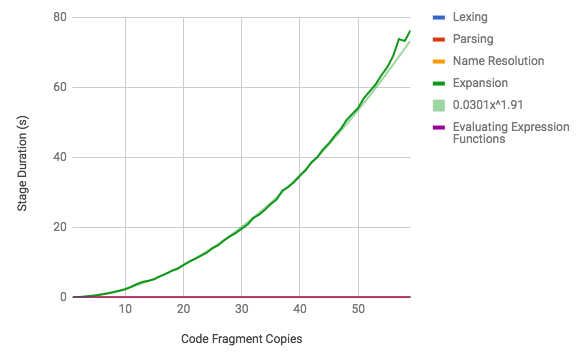
\includegraphics[width=\textwidth]{resources/performance-graph-with-expansion}
\caption{Phase runtime, the light green line is a best fit of the expansion phase}
\label{fig:performance-graph-with-expansion}
\end{figure}

\begin{listing}[t]
\begin{minted}{lua}
do
  function identity(x)
    return x
  end
end
\end{minted}
\caption{Simple Lua program that can be concatenated with itself without causing name errors.}
\label{lst:lua-fragment}
\end{listing}

We believe the slowness of expansion to not be an inherent property of the method, but rather a consequence of the simplest possible implementation. Expansion of a syntax construction assumes that each symbol exists at most once in binding position (see Section~\ref{sec:expansion-checking} for more information), and name resolution uses generated unique symbols and renaming to ensure this to be true. However, an expansion may duplicate one of its sub-nodes, which might produce a tree that has the same symbol in binding position multiple times.

Thus we reach the conclusion that we may need to perform name resolution after an expansion, to replace the duplicated binding symbols with distinct symbols.

The naive implementation of expansion thus expands a single syntax construction, then runs name resolution on the entire abstract syntax tree to ensure the invariant holds, then repeats, until no more syntax constructions can be expanded. This means that name resolution will be run roughly once per node in the syntax tree. Name resolution is at least linear in the size of the tree, since it examines every node. Thus the naive implementation is at least quadratic in the size of the syntax tree, which aligns pretty well with Figure~\ref{fig:performance-graph-with-expansion}.

However, most syntax constructions do not duplicate its sub-nodes. They are generally used at most once, in which case the extra name resolution pass is unnecessary. In fact, none of the syntax constructions used to implement the OCaml and Lua subsets use a sub-node more than once, thus the entire syntax tree could be expanded in a single bottom-up traversal. The extra work of a new name resolution pass between each individual expansion is thus quite significant.

\begin{figure}[t]
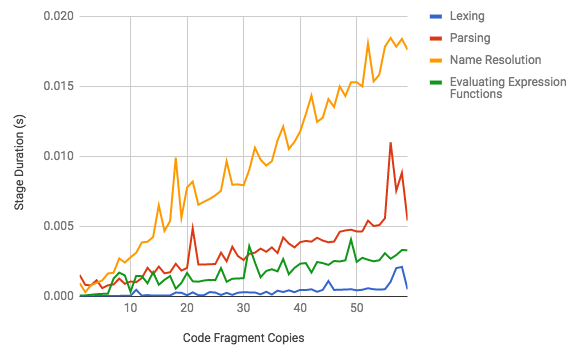
\includegraphics[width=\textwidth]{resources/performance-graph-without-expansion}
\caption{Stage runtime, excluding expansion}
\label{fig:performance-graph-without-expansion}
\end{figure}

As for the remaining parts of the implementation, Figure~\ref{fig:performance-graph-without-expansion} shows the runtime of each of the stages except expansion, for easier readability. Parsing requires an algorithm that can parse any context-free grammar and produce all syntax trees in case of ambiguities. The current implementation uses an off-the-shelf implementation\footnote{https://hackage.haskell.org/package/Earley} of the Earley \cite{Earley1970An-Efficient-Co} parsing algorithm. The algorithms used for grammar generation, expansion checking, expansion of a single instance (as opposed to full expansion of all instances), and name resolution have not been examined to determine time complexity, but have in practice had negligible impact on the run time of the implementation.

To summarize, the run time of the current implementation is dominated, by several orders of magnitude, by the expansion phase, which in the common case can be greatly optimized.

\section{Error Reporting} \label{sec:error-reporting}

Since one of the design goals is good error messages, this section examines the error messages produced by the implementation, and to some extent what the messages could be, given some more engineering and user experience effort.

Note that the errors examined are only those related to syntax constructions, i.e., ambiguous source code, incorrect expansions, and name binding errors. Errors that are not covered include type errors and runtime errors, since this thesis makes no contribution to either kind of error.

\subsection{Ambiguous Source Code} \label{sec:errors-ambiguous}

Syntax constructions provide no guarantee that a composed language has an unambiguous grammar. As such a user may write code that cannot be parsed unambiguously. At that point the user must be presented with a helpful error that can assist with solving the problem, without deep knowledge of the internals of the particular language, nor of grammars and parsing in general.

The error message should quickly direct the user to the actually ambiguous part of the code, and ideally also present what to change to select one of the possible interpretations.

\begin{listing}[t]
\begin{minted}{syncon}
syntax binaryAnd:Expression =
  a:Expression "&" b:Expression
{ <...> }
syntax binaryOr:Expression =
  a:Expression "|" b:Expression
{ <...> }
syntax variable:Expression =
  id:Identifier
{ <...> }
syntax parens:Expression =
  "(" e:Expression ")"
{ <...> }
\end{minted}
\begin{minted}{ocaml}
 a  &  b  |  c
(a  &  b) |  c
 a  & (b  |  c)
\end{minted}
\caption{Example of two operators without defined precedence, and the two interpretations}
\label{lst:undefined-precedence-operators}
\end{listing}

Listing~\ref{lst:undefined-precedence-operators} shows an example of two binary operators without defined precedence, requiring the user to explicitly group the operators. In this case the error produced will mark the correct part of the source code as ambiguous and present two different interpretations:

\begin{itemize}
  \item A \mintinline{syncon}{binaryOr} of a \mintinline{syncon}{binaryAnd} and a \mintinline{syncon}{variable}.
  \item A \mintinline{syncon}{binaryAnd} of a \mintinline{syncon}{variable} and a \mintinline{syncon}{binaryOr}.
\end{itemize}

It is worth noting that the current implementation shows the above information, plus the source code location of each mentioned syntax construction instance (both start and end), but the location information is here omitted for brevity and readability.

Ideally the system could detect that \mintinline{syncon}{parens} have no effect beyond grouping, and that it could be used to force one interpretation or the other, thus using it instead of the textual representation above, but that functionality is not present at the moment. As such the implementation will correctly identify the ambiguous section of the code, and provide a clear enough representation of the different ways to interpret the ambiguity, but no suggested changes are presented.

\begin{listing}[t]
\begin{minted}{syncon}
syntax sum:Expression =
  a:Expression "+" b:Expression
{
  #prec  11
  #assoc left
  <...>
}
syntax let:Expression =
  "let" x:Identifier args:Pattern*
  "=" e:Expression "in" body:Expression
{ <...> }
syntax bindingPattern:Pattern =
  id:Identifier
{ <...> }
syntax integerLiteral:Expression =
  i:Integer
{ <...> }
\end{minted}
\begin{minted}{ocaml}
 let x = 1 in  2  +  x
(let x = 1 in  2) +  x
 let x = 1 in (2  +  x)
\end{minted}
\caption{Example of a definition for a let expression leading to an ambiguous syntax, and an example with two interpretations}
\label{lst:ambiguous-let-expr}
\end{listing}

Listing~\ref{lst:ambiguous-let-expr} shows a definition of a \mintinline{ocaml}{let} expression used for a while during construction of the OCaml subset in Section~\ref{sec:functional-eval}. Since \mintinline{ocaml}{let} has no defined precedence it can both be a direct part of a sum (first interpretation in the example) and have a sum in its body (second interpretation in the example), without breaking precedence. The error presented marks the correct area of code, and presents two different interpretations:

\begin{itemize}
  \item A \mintinline{syncon}{sum} of a \mintinline{syncon}{let} and a \mintinline{syncon}{variable}.
  \item A \mintinline{syncon}{let} of a \mintinline{syncon}{bindingPattern}, an \mintinline{syncon}{integerLiteral} and a \mintinline{syncon}{sum}.
\end{itemize}

The latter interpretation is somewhat less obvious than the former, since we rarely think of a \mintinline{ocaml}{let} expression in terms of its nested syntactical elements, but the meaning is clear enough after comparing the interpretation with the offending source code.

It is worth noting here that parentheses could be used for disambiguation, similar to above, but the syntax of OCaml dictates that the code in Listing~\ref{lst:ambiguous-let-expr} should be unambiguously parsed as the second alternative. The solution in this case is to give \mintinline{ocaml}{let} a low precedence.

% TODO: write about [1; 2; 3]
\begin{listing}[t]
\begin{minted}{syncon}
syntax sequentialComposition:Expression =
  a:Expression ";" b:Expression
{
  #assoc right
  #prec 2
  <...>
}
syntax listLiteral:Expression =
  "[" (e:Expression (";" es:Expression)*)? "]"
{ <...> }
syntax variable:Expression =
  v:Identifier
{ <...> }
\end{minted}
\begin{minted}{ocaml}
[ a ; b ; c ]
[(a ; b ; c)]
[(a ; b); c ]
[ a ; b ; c ]
\end{minted}
\caption{Example of an ambiguous list literal. The alternative interpretations are presented as OCaml would parse them.}
\label{lst:ambiguous-list-literal}
\end{listing}

Listing~\ref{lst:ambiguous-list-literal} shows the list literal as originally implemented in the OCaml subset (see Section~\ref{sec:ambiguous-lists} for more details). The ambiguity occurs since the item separator in a list is the same as the sequential composition operator. The interpretations presented by the error message are as follows:

\begin{itemize}
  \item A sequence of a \mintinline{syncon}{sequentialComposition} and a \mintinline{syncon}{*} repetition covering no source code.
  \item A sequence of a \mintinline{syncon}{sequentialComposition} and a \mintinline{syncon}{*} repetition covering \mintinline{syncon}{; c}.
  \item A sequence of a \mintinline{syncon}{variable} and a \mintinline{syncon}{*} repetition covering \mintinline{syncon}{; b ; c}.
\end{itemize}

These interpretations expose rather more implementation details than the previous ones. A \mintinline{syncon}{sequence} refers to a parenthesized list of syntactical elements in a syntax description, i.e., \mintinline{syncon}{(e: Expression (";" es:Expression)*)} above. A \mintinline{syncon}{*} repetition refers to a syntactical element repeated using an EBNF operator, i.e., \mintinline{syncon}{(";" es:Expression)*} above.

The \mintinline{syncon}{sequence} is reported instead of \mintinline{syncon}{listLiteral} since, implementation-wise, it is the closest node in the syntax tree that covers the entire ambiguity. The \mintinline{syncon}{listLiteral} also covers the square brackets, but those are parsed unambiguously. The repetition is reported as such instead of some number of \mintinline{syncon}{variable}s simply because it was the easiest information to obtain given the current implementation.

A language implementer might appreciate the above representations of the interpretations, while an end user would most likely rather want the closest enclosing syntax construction and a list of its child syntax constructions, regardless of internal structure of the syntax construction and it possibly covering some unambiguous parts of the code.

Since ambiguity reporting identifies the minimal subtrees that are ambiguous, either representation is simple to obtain. The user could thus potentially choose their own preference, depending on whether they are an end user or a language implementer.

\subsubsection{Static and Dynamic Ambiguity Detection} \label{sec:static-dynamic-ambiguity}

% TODO: link this to the previous section properly, i.e. transition into a question on how to ensure the correctness of a language implementation syntax-wise, and how that question is somewhat close to 'normal' static vs dynamic type checking and what constitutes correct there
The errors presented above bear something of a resemblance  to runtime errors in a dynamic programming language, i.e., a programming language without compile time type checking: an ambiguous language only produces errors at parse-time and an incorrect program only produces errors at run-time.

Correctness in a dynamically typed language tends to depend more on testing, manual or automated, than static guarantees, since the latter are largely absent. Testing for ambiguity is rather straightforward, merely provide example code and state whether it is ambiguous or not, then try parsing it.

However, ambiguity is generally a property of a set of syntax constructions, not of any syntax construction in itself. Passing tests for one set of syntax constructions (i.e. a language) give little to no information for another set, even if the two intersect (i.e., they share syntax constructions). Thus a complete set of tests need to be created for each language.

This is analogous to integration tests in a dynamically typed language; a new system (i.e., a new composition of sub-systems) require new integration tests. However, regular programming languages additionally tend to have unit tests, which tests some unit of the program (e.g., a function) independently of the rest of the program. These tests give useful results about the tested units even when they are composed into a bigger system. Testing syntax construction languages for ambiguity has no corresponding concept, thus requiring the testing process to essentially start from scratch for every new language.

Static ambiguity detection on the other hand, i.e., compile-time checking, would alleviate this effort greatly, since it would be automatic and ideally complete for each language without extra work for the language designer. This thesis makes no attempt at determining the ambiguity of a language, instead leaving such an approach for future work.

\subsection{Expansion Specification Errors}

The tool implemented for this thesis performs the checking necessary to ensure that no syntax construction has an expansion that may produce a malformed syntax tree. The errors presented when such an expansion is encountered are informative, but no effort has been put into making the presentation user friendly. Keeping that in mind, the errors presented are one of the following:

\begin{description}
  \item[Missing export] The syntax construction specifies \mintinline{syncon}{#bind x before} or \mintinline{syncon}{#bind x after}, but the expansion does not expose \mintinline{syncon}{x}. This error is also produced if a syntax construction appears in the top-level scope in the syntax construction before expansion, but is in an inner scope or not present after expansion, since it could also export a symbol.

  \item[Dependency error] The checker uses a concept of a dependency, which is either an \mintinline{syncon}{Identifier} or a syntax construction along with a direction (before or after). These define the sources from which a reference may find its binding. Since any of these sources may be used the dependency set of a syntax construction after expansion must be a superset of its dependency set before expansion.

  \item[Self dependency] Following the definition of a dependency above, if a syntax construction depends on itself (i.e., on a copy of itself) after expansion, and it binds a symbol, then this symbol is defined (at least) twice. Technically this is only an error if at least two of the definitions are in the same scope, shadowing is allowed as long as it is in a child scope, but the implementation is currently slightly overly cautious and rejects any self dependency.

  \item[Binding error] Since an expansion can use any syntax in its definition it may also introduce new bindings and identifiers. These are checked the same as normal name resolution and reported in a similar fashion.
\end{description}

Note that the expansion checking is performed on a single syntax construction, entirely independent of other syntax constructions or source code to parse.

The errors are presented in terms of hypothetical syntax trees with the syntax construction being checked as the root. References to elements in this tree are by position in the tree, since not all things are named in the syntax description and even things that are named might be duplicated because of an EBNF operator.

As a non-trivial example, consider this implementation of an \mintinline{lua}{if}-statement (from the Lua implementation in Section~\ref{sec:imperative-eval}). The expansion uses the core language builtin \mintinline{syncon}{#if}, which requires the two branches to be single argument functions that are passed \mintinline{syncon}{#unit} if they are chosen for execution.

\begin{minted}[linenos]{syncon}
syntax if:Statement =
  "if" cond:Expression
  "then" then:Block
  elseif:("elseif" econd:Expression
          "then" ethen:Block)*
  ("else" else:Block)? "end"
{
  #scope (then)
  #scope elseif:(ethen)
  #scope (else)

  BExpression`
    efun return. efun break. #if (#deref `t(cond))
      (fun _. `t(then) return break)
      (fun _. `t(
        foldr elseif next
          (BExpression` #if (#deref `t(econd))
            (fun _. `t(ethen) return break)
            (fun _. `t(next)))
        foldr else _
          (BExpression` `t(else) return break)
        (BExpression` #unit)))
}
\end{minted}

Expansion checking produces several errors, here slightly abbreviated and clarified, and further explained and summarized later:
\begin{enumerate}
  \item \mintinline{syncon}{syntax#[1]} needs \mintinline{syncon}{before} exports from \mintinline{syncon}{syntax#[4,0,1]}.
  \item \mintinline{syncon}{syntax#[1]} needs \mintinline{syncon}{before} exports from \mintinline{syncon}{syntax#[4,1,1]}.
  \item \mintinline{syncon}{syntax#[3]} needs \mintinline{syncon}{before} exports from \mintinline{syncon}{syntax#[4,0,1]}.
  \item \mintinline{syncon}{syntax#[3]} needs \mintinline{syncon}{before} exports from \mintinline{syncon}{syntax#[4,1,1]}.
  \item \mintinline{syncon}{syntax#[4,0,1]} needs \mintinline{syncon}{before} exports from \mintinline{syncon}{syntax#[4,1,1]}.
  \item \mintinline{syncon}{syntax#[4,0,3]} needs \mintinline{syncon}{before} exports from \mintinline{syncon}{syntax#[4,1,1]}.
  \item \mintinline{syncon}{syntax#[4,0,1]} \mintinline{syncon}{before} exports should be exported.
  \item \mintinline{syncon}{syntax#[4,0,1]} \mintinline{syncon}{after} exports should be exported.
  \item \mintinline{syncon}{syntax#[4,1,1]} \mintinline{syncon}{before} exports should be exported.
  \item \mintinline{syncon}{syntax#[4,1,1]} \mintinline{syncon}{after} exports should be exported.
\end{enumerate}

The \mintinline{syncon}{syntax#[<...>]} expressions refer to elements in the syntax tree using the path concept introduced in Chapter~\ref{sec:formalization}. Note, however, that the paths in the implementation are zero-indexed, while the formalization refers to them as one-indexed. For example, \syncon{syntax#[4,0,1]} refers to the first repetition of \syncon{econd} (on line~4). We can see this by noting that the element with index \syncon{4} in the syntax description is \syncon{elseif:(<...>)*}, whose child with index \syncon{0} is \syncon{elseif:(<...>)} (note the absence of \syncon{*}), whose child with index \syncon{1} is \syncon{econd:Expression}. Similarly, \syncon{syntax#[4,1,1]} also refers to \syncon{econd}, but in the second repetition of \syncon{elseif}.

Using this information we can summarize the errors to the following list:

\begin{enumerate}
  \item \mintinline{syncon}{cond} needs \mintinline{syncon}{before} exports from \mintinline{syncon}{econd}. (1, 2)
  \item \mintinline{syncon}{then} needs \mintinline{syncon}{before} exports from \mintinline{syncon}{econd}. (3, 4)
  \item \mintinline{syncon}{econd} needs \mintinline{syncon}{before} exports from later repetitions of \mintinline{syncon}{econd}. (5)
  \item \mintinline{syncon}{ethen} needs \mintinline{syncon}{before} exports from later repetitions of \mintinline{syncon}{econd}. (6)
  \item Both \mintinline{syncon}{before} and \mintinline{syncon}{after} exports from \mintinline{syncon}{econd} need to be re-exported. (7-10)
\end{enumerate}

The errors arise because the expansion puts repetitions of \mintinline{syncon}{econd} inside functions, later repetitions nested further in, which restricts their exports, hiding them from most preceding elements as well as the surrounding syntax tree.

To solve this we wrap the conditions in their own scope and restrict their exports before expansion; we most likely do not intend for variables bound in the condition to be visible outside of the if-statement.

The errors presented here are perhaps not particularly nice to read or understand, but they contain the information needed to construct better messages, it ''just'' requires some more engineering and user experience effort.

\subsection{Binding Errors}

The errors presented by the implementation in the presence of binding errors add nothing new beyond what is common in most compilers. The following errors are reported:

\begin{description}
  \item[Undefined symbol] If an identifier is encountered in a non-binding position and no binding with the same symbol is in scope this error is reported, along with the source code location of the unresolved identifier.

  \item[Symbol already defined] Bindings may shadow bindings from outer scopes, but if a symbol is defined twice in the same scope, and the bindings cover an overlapping area of code, then this error is reported. The source code location of both definitions are included.

  The overlapping requirement is important: a binding that can be used both before and after its definition is defined by using both \mintinline{syncon}{#bind x before} and \mintinline{syncon}{#bind x after}. This binds the same symbol twice in the same scope, but since the bound areas do not overlap, no error is reported.
\end{description}

% TODO: this sentence is not very clear to most I think
Since all errors are independent in the sense that none of them is the cause of any other, they can all be collected and presented to the user at once.

No binding errors can be encountered during expansion of syntax construction, nor when all syntax constructions are expanded, thus all binding errors are reported in terms of the original source code written by the end user.

\chapter[Limitations, Future Work, and Conclusion]{Limitations, Future Work,\\and Conclusion}

This chapter summarizes the limitations discovered during evaluation, suggests potential improvements for future work, and concludes by comparing the results with the design goals introduced in Section~\ref{sec:research-question}.

\section{Limitations and Future Work}

The limitations discussed in Chapter~\ref{sec:evaluation}, and the future work they each suggest, can be grouped into the following categories:

\begin{description}
  \item[Contextual Information] Certain programming language features require information specified by their context without a programmer using an explicit reference to that context, for example, a \mintinline{lua}{break} statement must abort the innermost surrounding loop without any reference to it. Other examples of this can be found in sections \ref{sec:imperative-eval} (\mintinline{lua}{break} and \mintinline{lua}{return}) and \ref{sec:functional-eval} (pattern matching). Syntax constructions have no concept of this, it is instead implemented using either regular functions in the core language, or expression functions, introduced in Section~\ref{sec:core-language}. However, as elaborated later in the same section (starting on page \pageref{sec:efun-drawbacks}), these cannot be correctly described using syntax constructions, thus the expansion checker cannot guarantee an expansion's correctness. Additionally, they unnecessarily couple the implementation of different syntax constructions to each other.

  A better solution for future work may be to create a form of lexical bindings, where a syntax construction may set the value of such a binding for all its descendants, and a syntax construction that uses such a binding may not be used where it is unset (e.g., \mintinline{lua}{break} may only be used inside a loop, which would set such a binding).

  \item[Ambiguity Control] Syntax constructions allow for ambiguity in the syntax of a programming language where desired, but provides poor control over it. The language designer gets no help in ensuring its presence or absence but must instead test for it themselves. Additionally, when ambiguity is present but undesired the tools to remove it are frequently not very convenient, page~\pageref{sec:lua-func-call-precedence} for example contains an unintentional ambiguity with a slightly inconvenient solution, while page~\pageref{sec:ambiguous-lists} contains an unintentional ambiguity with a significantly inconvenient solution.

  Future work must here come in two different, but related flavors:
  \begin{itemize}
    \item Control of where ambiguity appears. This requires static analysis of the grammar, which in the general case is is undecidable for a context-free grammar \cite{Cantor1962On-The-Ambiguit}. The question then becomes if a heuristic is sufficient, or if some more restricted form of grammar can support the desired workflow of defining the syntax of each syntax construction separately.

    % TODO: the suggested future work things here might not be well described, and might be too specific? Should they truly be here in this fashion?
    \item Tools to remove or add ambiguity. Precedence as a number easily turns unwieldy, and turns out to be insufficiently flexible (e.g., see p.~\pageref{sec:ambiguous-lists}). Disallowing specific syntax constructions from appearing in certain positions would solve this particular problem (the expressions in a list literal cannot be sequential composition), and may prove to be a more flexible tool.
  \end{itemize}

  \item[Separated Symbol Domains] All bound symbols are treated the same by syntax constructions, but many languages partition them into groups, a common example being the separation of types from values: names bound as types are fully separated from names bound as values. % TODO: ref to place where this is discussed?

  \item[Disambiguation by binding or reference] Some programming languages have features that behave differently depending on whether an identifier is previously bound or not. Page~\pageref{sec:prolog-pattern-matching} discusses this in more detail, but the most natural way to express this with syntax constructions is to define two syntax constructions, one for when the identifier is bound and one for when it is not, but otherwise syntactically identical, which the system as it stands cannot handle unambiguously.

  \item[Namespaces] Though explicitly ignored in this thesis (see delimitations in Section~\ref{sec:delimitations}), namespaces and the ability to import definitions from them are important parts of many programming languages and should play a part in future work.

  \item[Performance] The current implementation has an inefficient expansion phase. However, as discussed in Section~\ref{sec:performance}, we believe that a very large portion of the work performed is unnecessary; only the syntax constructions that duplicate a subtree might require an extra name resolution pass after expansion. Future work could thus likely greatly improve performance in the common case by tracking potential duplication, and omitting the name resolution pass when possible.
\end{description}

\section{Conclusion}

This thesis has presented a first attempt at a method for defining programming languages through individual features, allowing reuse and composition of much smaller parts than entire languages.

Evaluating based on the design goals stated after the initial problem statement (see Section~\ref{sec:research-question}) we find the following:

\begin{description}
  \item[Tower of languages:] A syntax construction defines its implementation in terms of some other language, using the syntax of that language. However, the inability to treat subexpressions in a non-atomic way somewhat limit their expressive power compared to the macros commonly found in Lisp dialects.

  \item[Syntactical freedom:] A language can express essentially any context-free grammar, thus the syntactical freedom is far greater than for example Lisp or C. However, the fixed tokenization precludes customization of for example comments or identifiers, and the rewrites required to avoid undesired ambiguity are sometimes significant.

  \item[Abstraction preservation:] The expansion checker has not allowed any abstraction breaking expansions in practice, and the justification presented in the formalization appears sound.

  \item[Good error messages:] The error messages presented are informative and specific, though more engineering work is required to make them truly palatable.

  \item[Composition through cherry-picking:] Though technically doable, certain common situations make the resulting language ambiguous, requiring creating a new syntax construction simply to wrap the imported one. This boilerplate seems undesirable, but a better solution is left for future work.

  \item[Reasoning without context:] The \syncon{#precedence} declaration present in some syntax constructions present an implicit dependency on all other syntax constructions with a declared precedence. Additionally, the rewrites mentioned earlier require changing or creating several syntax constructions in tandem, i.e., they must be considered in their context. A majority of the syntax constructions defined could however be considered without context.
\end{description}

Syntax constructions thus do not fully meet the goals initially presented, but they do provide a reasonable first step.

\printbibliography[heading=bibintoc]

\appendix

\chapter[Language Definition: Formalization Core]{Language Definition:\\Formalization Core} \label{sec:formal-core}

\inputminted{syncon}{implementation/languages/formalization-example/core}

\chapter[Language Definition: OCaml Subset]{Language Definition:\\OCaml Subset} \label{sec:appendix-ocaml}

\inputminted{syncon}{implementation/languages/ocaml/language}

\chapter[Language Definition: Lua Subset]{Language Definition:\\Lua Subset} \label{sec:appendix-lua}

\inputminted{syncon}{implementation/languages/lua/language}

\end{document}
